%%%%%%%%%%%%%%%%%%%%%%%%%%%%%%%%%%%%%%%%%%%%%%%%%%%%%%%%%%%%%%%%%%%%%%
% Overleaf (WriteLaTeX) Example: Molecular Chemistry Presentation
%
% Source: http://www.overleaf.com
%
% In these slides we show how Overleaf can be used with standard 
% chemistry packages to easily create professional presentations.
% 
% Feel free to distribute this example, but please keep the referral
% to overleaf.com
% 
%%%%%%%%%%%%%%%%%%%%%%%%%%%%%%%%%%%%%%%%%%%%%%%%%%%%%%%%%%%%%%%%%%%%%%
% How to use Overleaf: 
%
% You edit the source code here on the left, and the preview on the
% right shows you the result within a few seconds.
%
% Bookmark this page and share the URL with your co-authors. They can
% edit at the same time!
%
% You can upload figures, bibliographies, custom classes and
% styles using the files menu.
%
% If you're new to LaTeX, the wikibook is a great place to start:
% http://en.wikibooks.org/wiki/LaTeX
%
%%%%%%%%%%%%%%%%%%%%%%%%%%%%%%%%%%%%%%%%%%%%%%%%%%%%%%%%%%%%%%%%%%%%%%

\documentclass{beamer}

% For more themes, color themes and font themes, see:
% http://deic.uab.es/~iblanes/beamer_gallery/index_by_theme.html
%
\mode<presentation>
{
  \usetheme{Madrid}       % or try default, Darmstadt, Warsaw, ...
  \usecolortheme{default} % or try albatross, beaver, crane, ...
  \usefonttheme{serif}    % or try default, structurebold, ...
  \setbeamertemplate{navigation symbols}{}
  \setbeamertemplate{caption}[numbered]
} 

\usepackage[portuguese]{babel}
\usepackage[utf8x]{inputenc}
\usepackage{chemfig}
\usepackage[version=3]{mhchem}


% On Overleaf, these lines give you sharper preview images.
% You might want to `comment them out before you export, though.
\usepackage{pgfpages}
\pgfpagesuselayout{resize to}[%
  physical paper width=8in, physical paper height=6in]

% Here's where the presentation starts, with the info for the title slide
\title[]{Projeto de Fundamentos de IoT \\Vagas no Estacionamento}
\author{Reynaldo Caceres Villena}
\institute{IME-USP}
\date{Junho - 2018}

\begin{document}

\begin{frame}{}
  \maketitle
\end{frame}

\begin{frame}{}
  \tableofcontents
\end{frame} 

\section{Introdução}
\begin{frame}{Introdução}
  \begin{block}{}
   \begin{center}
Vagas no Estacionamento    
   \end{center}  
  \end{block}
   \begin{center}
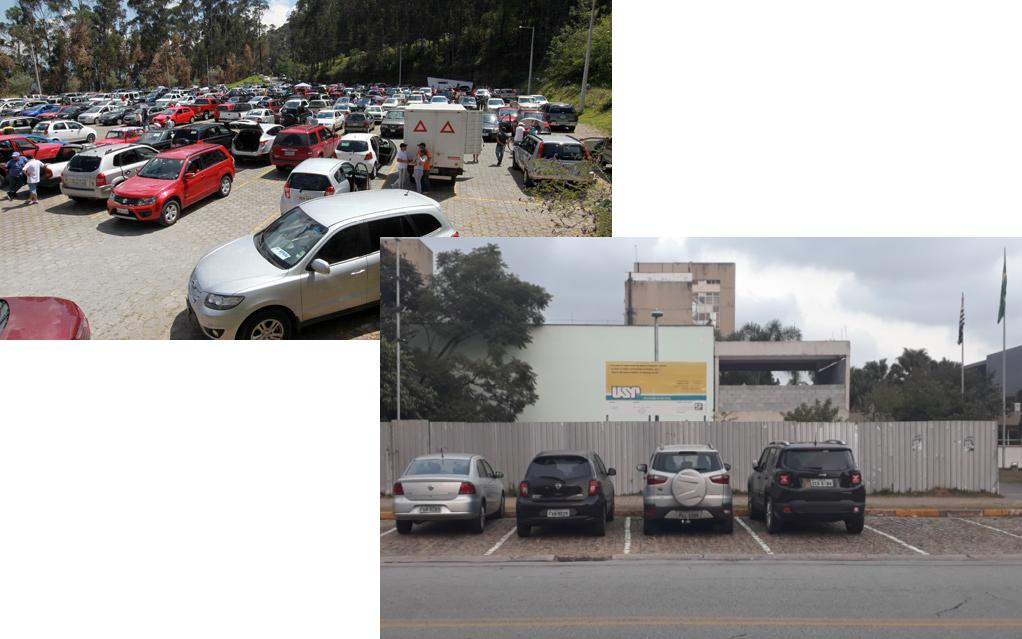
\includegraphics[width=.8\textwidth]{img/slide_1.jpeg}  
   \end{center}  

\end{frame}


\begin{frame}{}
  \tableofcontents
\end{frame}

\section{Estrutura de Projeto}
\subsection{Aparelhos}
\subsubsection{Raspberry Pi 3 Model B}

\begin{frame}{Aparelhos}

\begin{exampleblock}{}
   \begin{center}
    Raspberry Pi 3 Model B    
   \end{center}
\end{exampleblock}   
\begin{center}
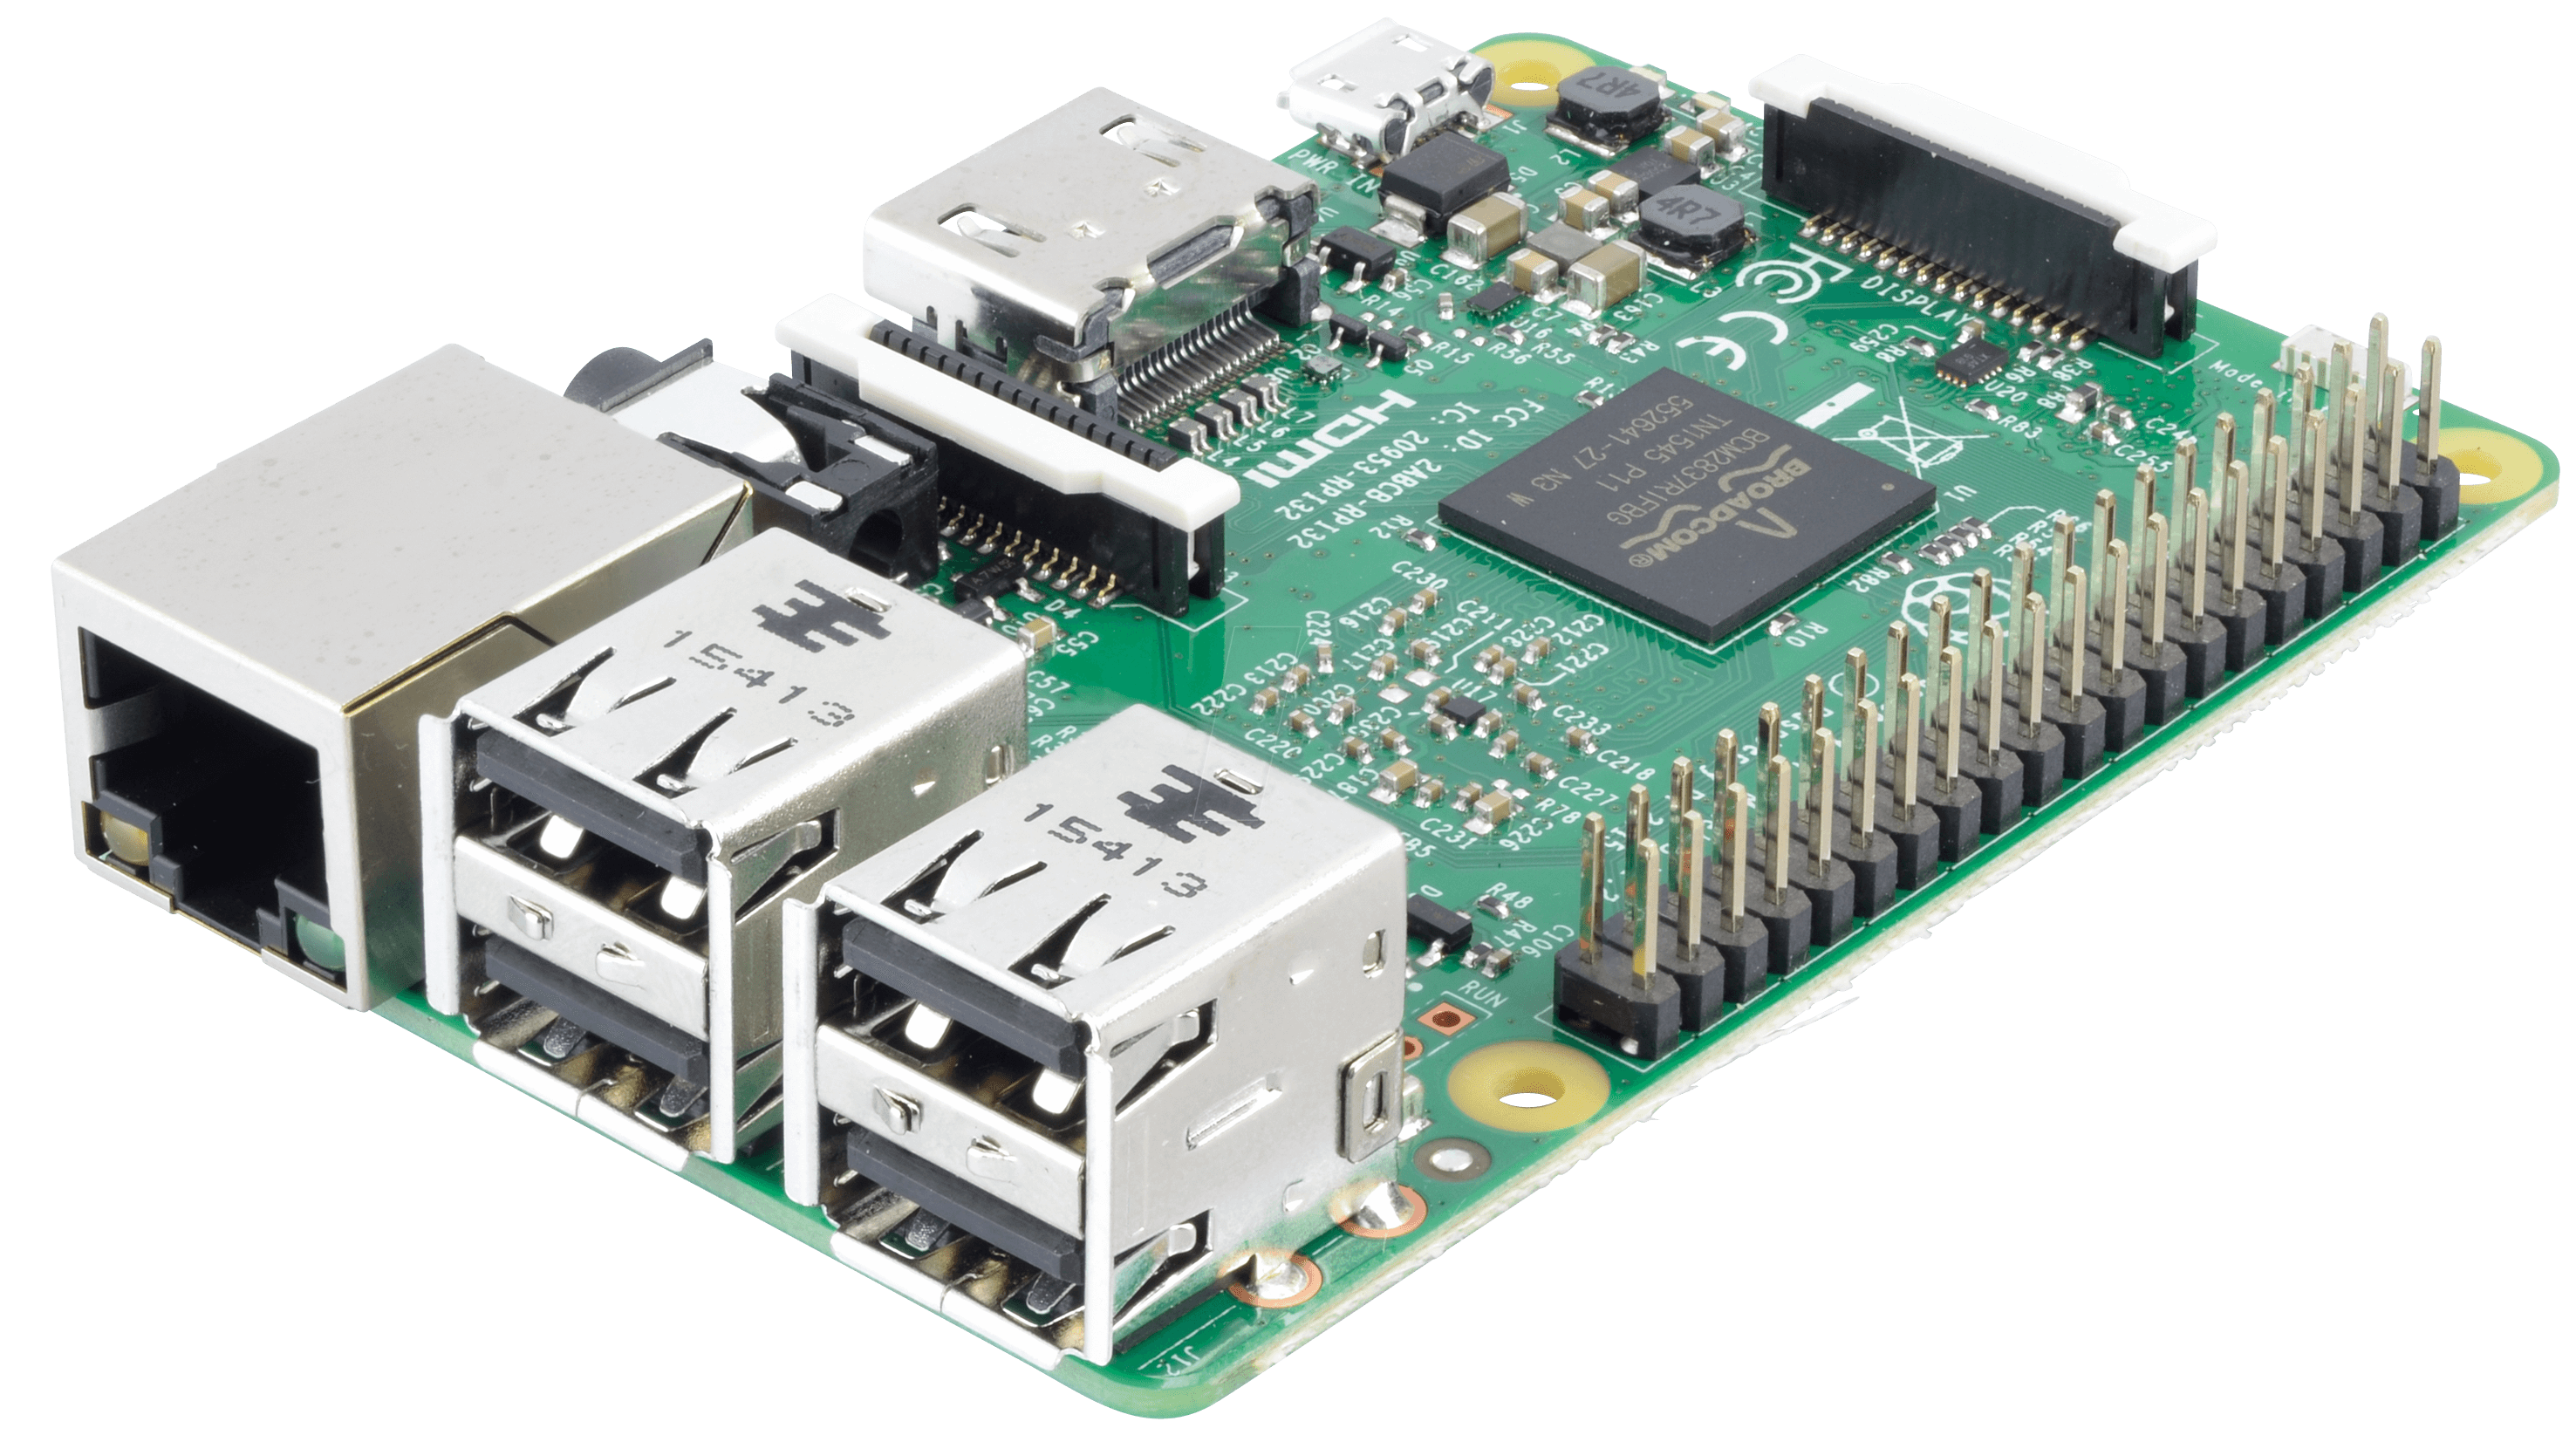
\includegraphics[width=.56\textwidth]{img/slide_rasp1.png}   
\end{center}

\begin{columns}
\begin{column}{0.56\textwidth}
\begin{itemize}\tiny
 \item A 1.2GHz 64-bit quad-core ARMv8 CPU
 \item 802.11n Wireless LAN
 \item Bluetooth 4.1 \& Bluetooth Low Energy (BLE)
 \item 1GB RAM
 \item 10/100 Ethernet port
 \item 802.11n WiFi NIC
 \item Bluetooth 4.1 \& Bluetooth Low Energy (BLE)
\end{itemize}
\end{column}
\begin{column}{0.44\textwidth}
\begin{itemize}\tiny
 \item HDMI port
 \item USB 2.0 interface x 4
 \item Micro SD card slot
 \item 40-pin GPIO interface
 \item Camera interface (CSI)
 \item Display interface (DSI)
 \item Upgraded power management
 \item supports more peripherals  
 \end{itemize}
\end{column}
\end{columns}

\end{frame}




\subsubsection{Câmeras}

\begin{frame}{Aparelhos}

\begin{exampleblock}{}
   \begin{center}
    Câmeras    
   \end{center}
\end{exampleblock}   

\begin{columns}
\begin{column}{0.5\textwidth}
\begin{center}
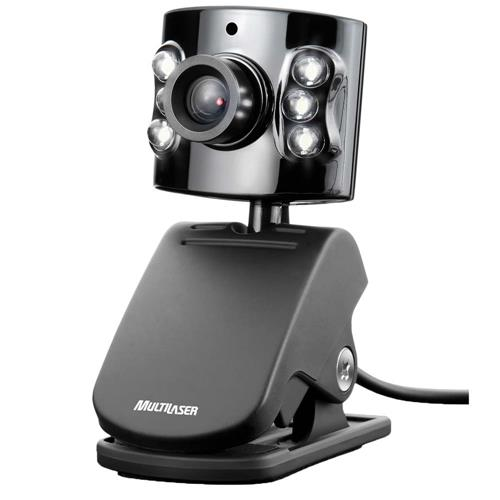
\includegraphics[width=.56\textwidth]{img/slide_cam1.jpeg}   
\end{center}
Camera Multilaser WC040
\begin{itemize}\tiny
 \item Vídeos de 1.3 Mpx (1280 x 1024 pixels)
 \item Fotos de 5 Mpx (via interpolação) 
 \item Conexão direta (USB).
\end{itemize}
\end{column}
\begin{column}{0.5\textwidth}
\begin{center}

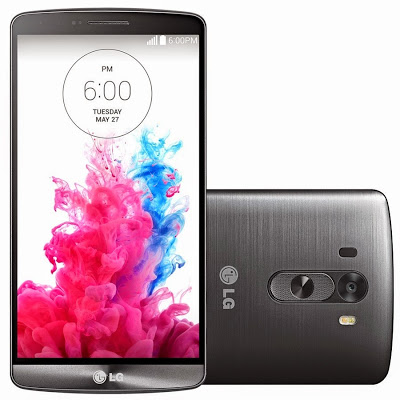
\includegraphics[width=.56\textwidth]{img/slide_cam2.jpg}   
\end{center}
Celular LG G3
\begin{itemize}\tiny
 \item Vídeos em 4K (3840x2160 pixels)  
 \item Fotos de 13 Mpx (4160x3120 pixels) 
 \item Conexão via LAN (aplicativo IP Webcam)
\end{itemize}
\end{column}
\end{columns}
\end{frame}

\subsection{Serviços}
\subsubsection{Computer Visual API- Azure}

\begin{frame}{Serviços}

\begin{exampleblock}{}
   \begin{center}
   Computer Vision API
   \end{center}
\end{exampleblock}
Mycrosoft Azure (https://azure.microsoft.com/en-us/services/)   

\begin{center}
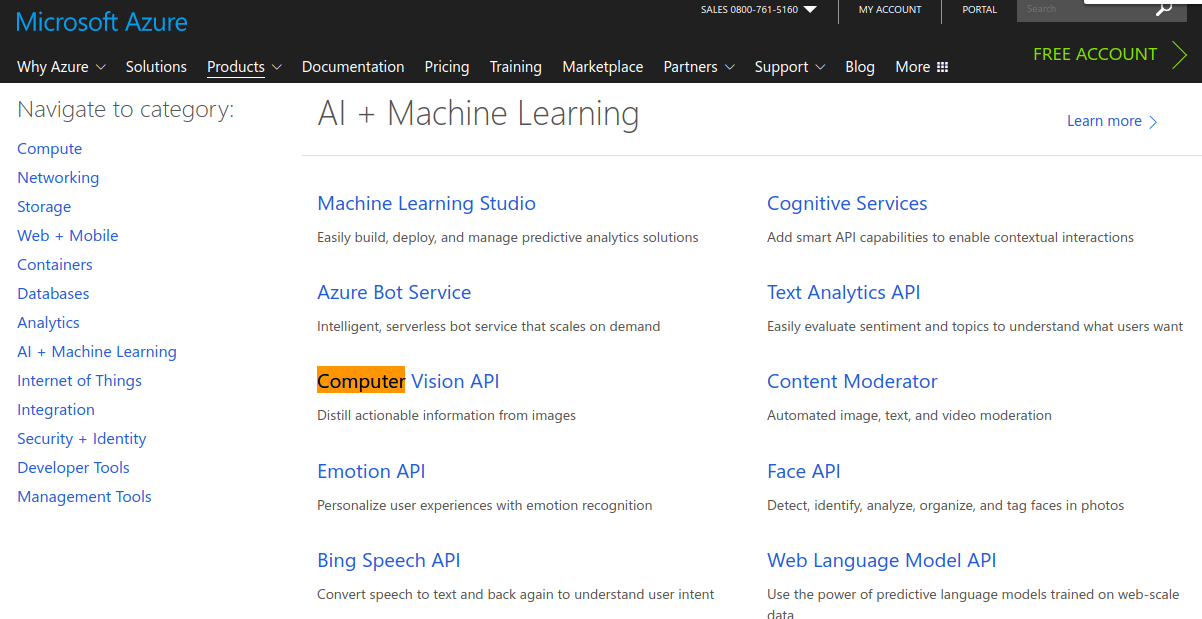
\includegraphics[width=.8\textwidth]{img/Azuri.png}   
\end{center}
\begin{itemize}\tiny
\item Computer Vision API tem um conjunto de algoritmos que
processam as imagens e devolvem certa informação.
\end{itemize}

\end{frame}





\begin{frame}{Serviços}

\begin{exampleblock}{}
   \begin{center}
   Computer Vision API
   \end{center}
\end{exampleblock}

\begin{columns}
\begin{column}{0.5\textwidth}
\begin{center}
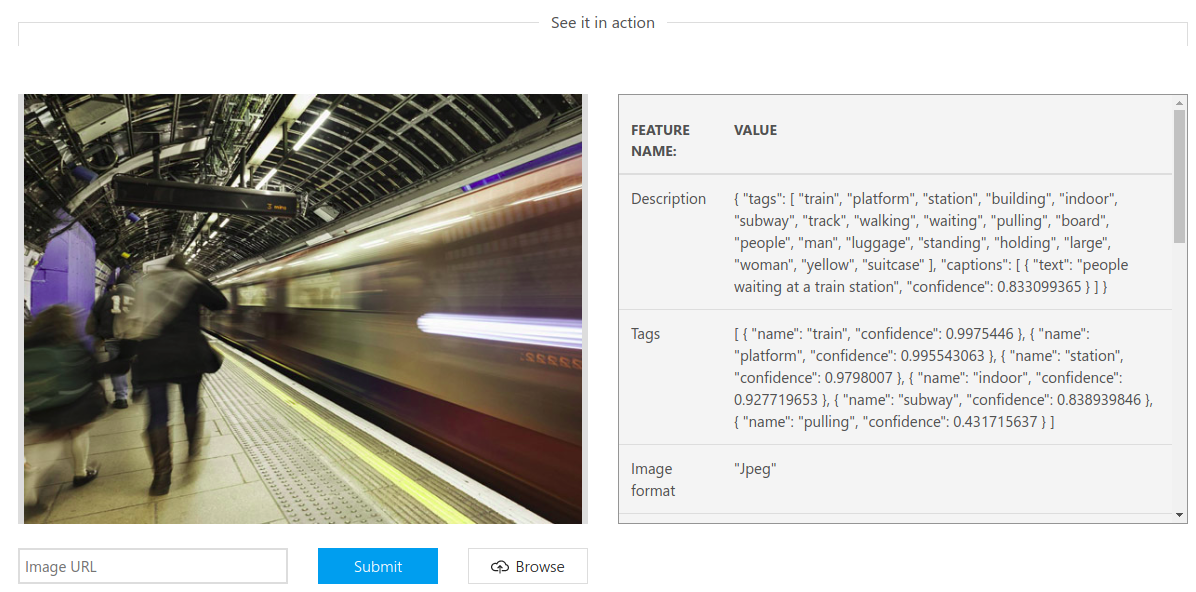
\includegraphics[width=1\textwidth]{img/Azuri_1.png}   

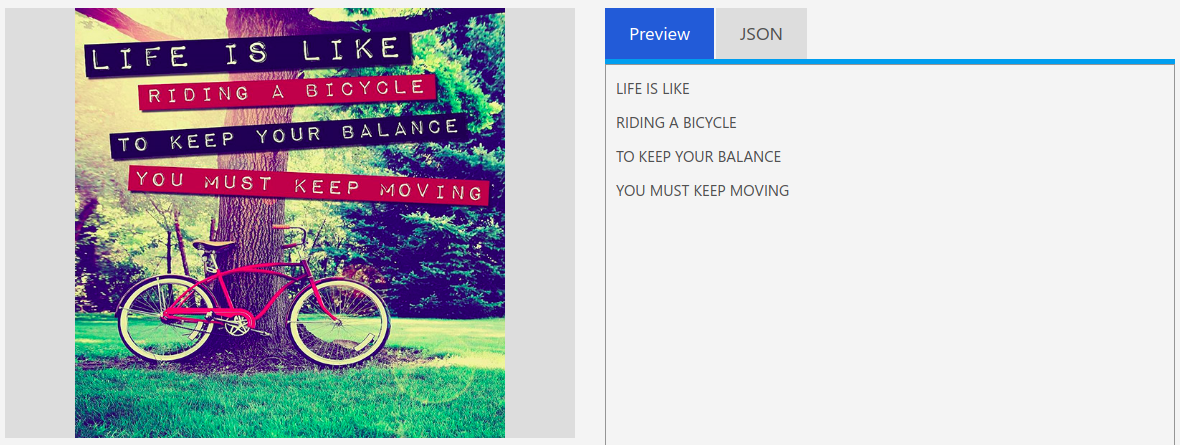
\includegraphics[width=1\textwidth]{img/Azuri_3.png}   
\end{center}
\end{column}
\begin{column}{0.5\textwidth}
\begin{center}
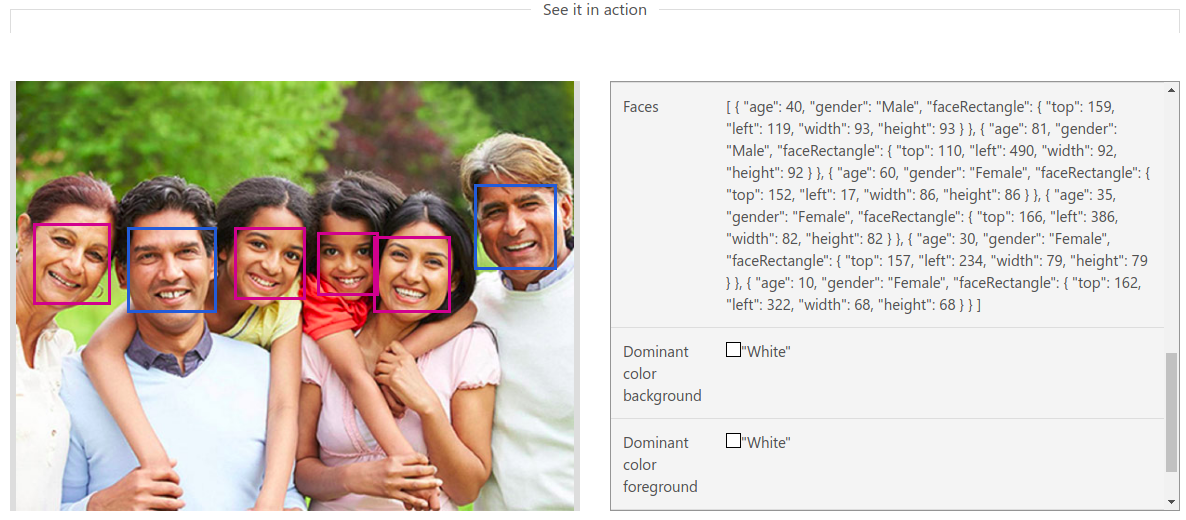
\includegraphics[width=1\textwidth]{img/Azuri_2.png}   

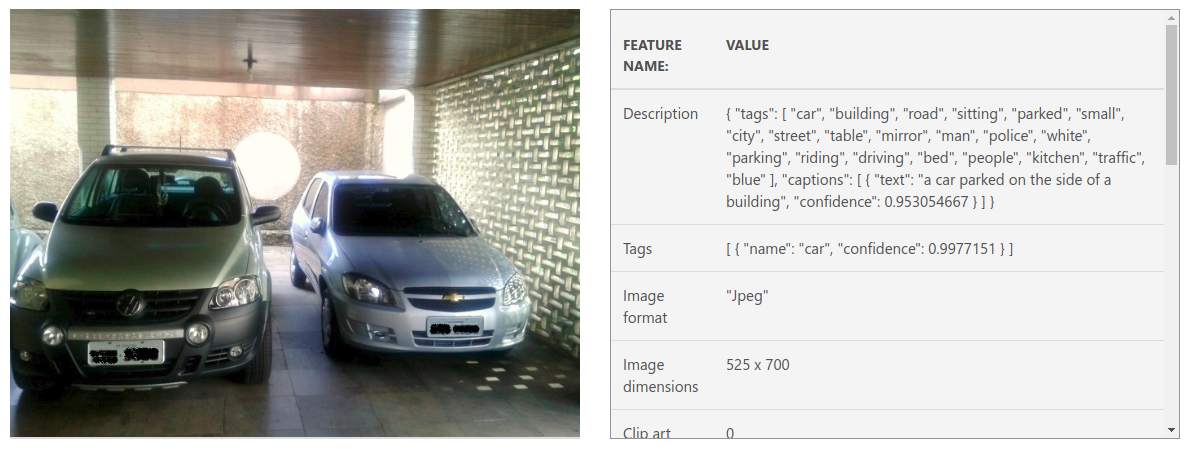
\includegraphics[width=1\textwidth]{img/Azuri_4.png}   
\end{center}
\end{column}
\end{columns}
\end{frame}













\subsubsection{Pythonanywhere}

\begin{frame}{Serviços}

\begin{exampleblock}{}
   \begin{center}
   Pythonanywhere
   \end{center}
\end{exampleblock}
https://www.pythonanywhere.com/
\begin{center}

\includegraphics[width=1\textwidth]{img/pythonanywhere.png}  
\end{center}
\begin{columns}
\begin{column}{0.4\textwidth}
\begin{center}

\includegraphics[width=1\textwidth]{img/pythonanywhere_flask.png}   
\end{center}
\end{column}
\begin{column}{0.6\textwidth}
\begin{itemize}\tiny
 \item Ambiente de desenvolvimento integrado (IDE)
 \item Serviço de hospedagem web  
\end{itemize}
\begin{center}
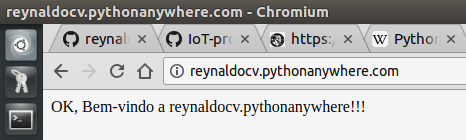
\includegraphics[width=.6\textwidth]{img/pythonanywhere_rey.png}    
\end{center}
\end{column}
\end{columns}
\end{frame}


\subsubsection{Linguagens de Programação }

\begin{frame}{Linguagens de Programação}


\begin{columns}
\begin{column}{0.3\textwidth}
\begin{center}
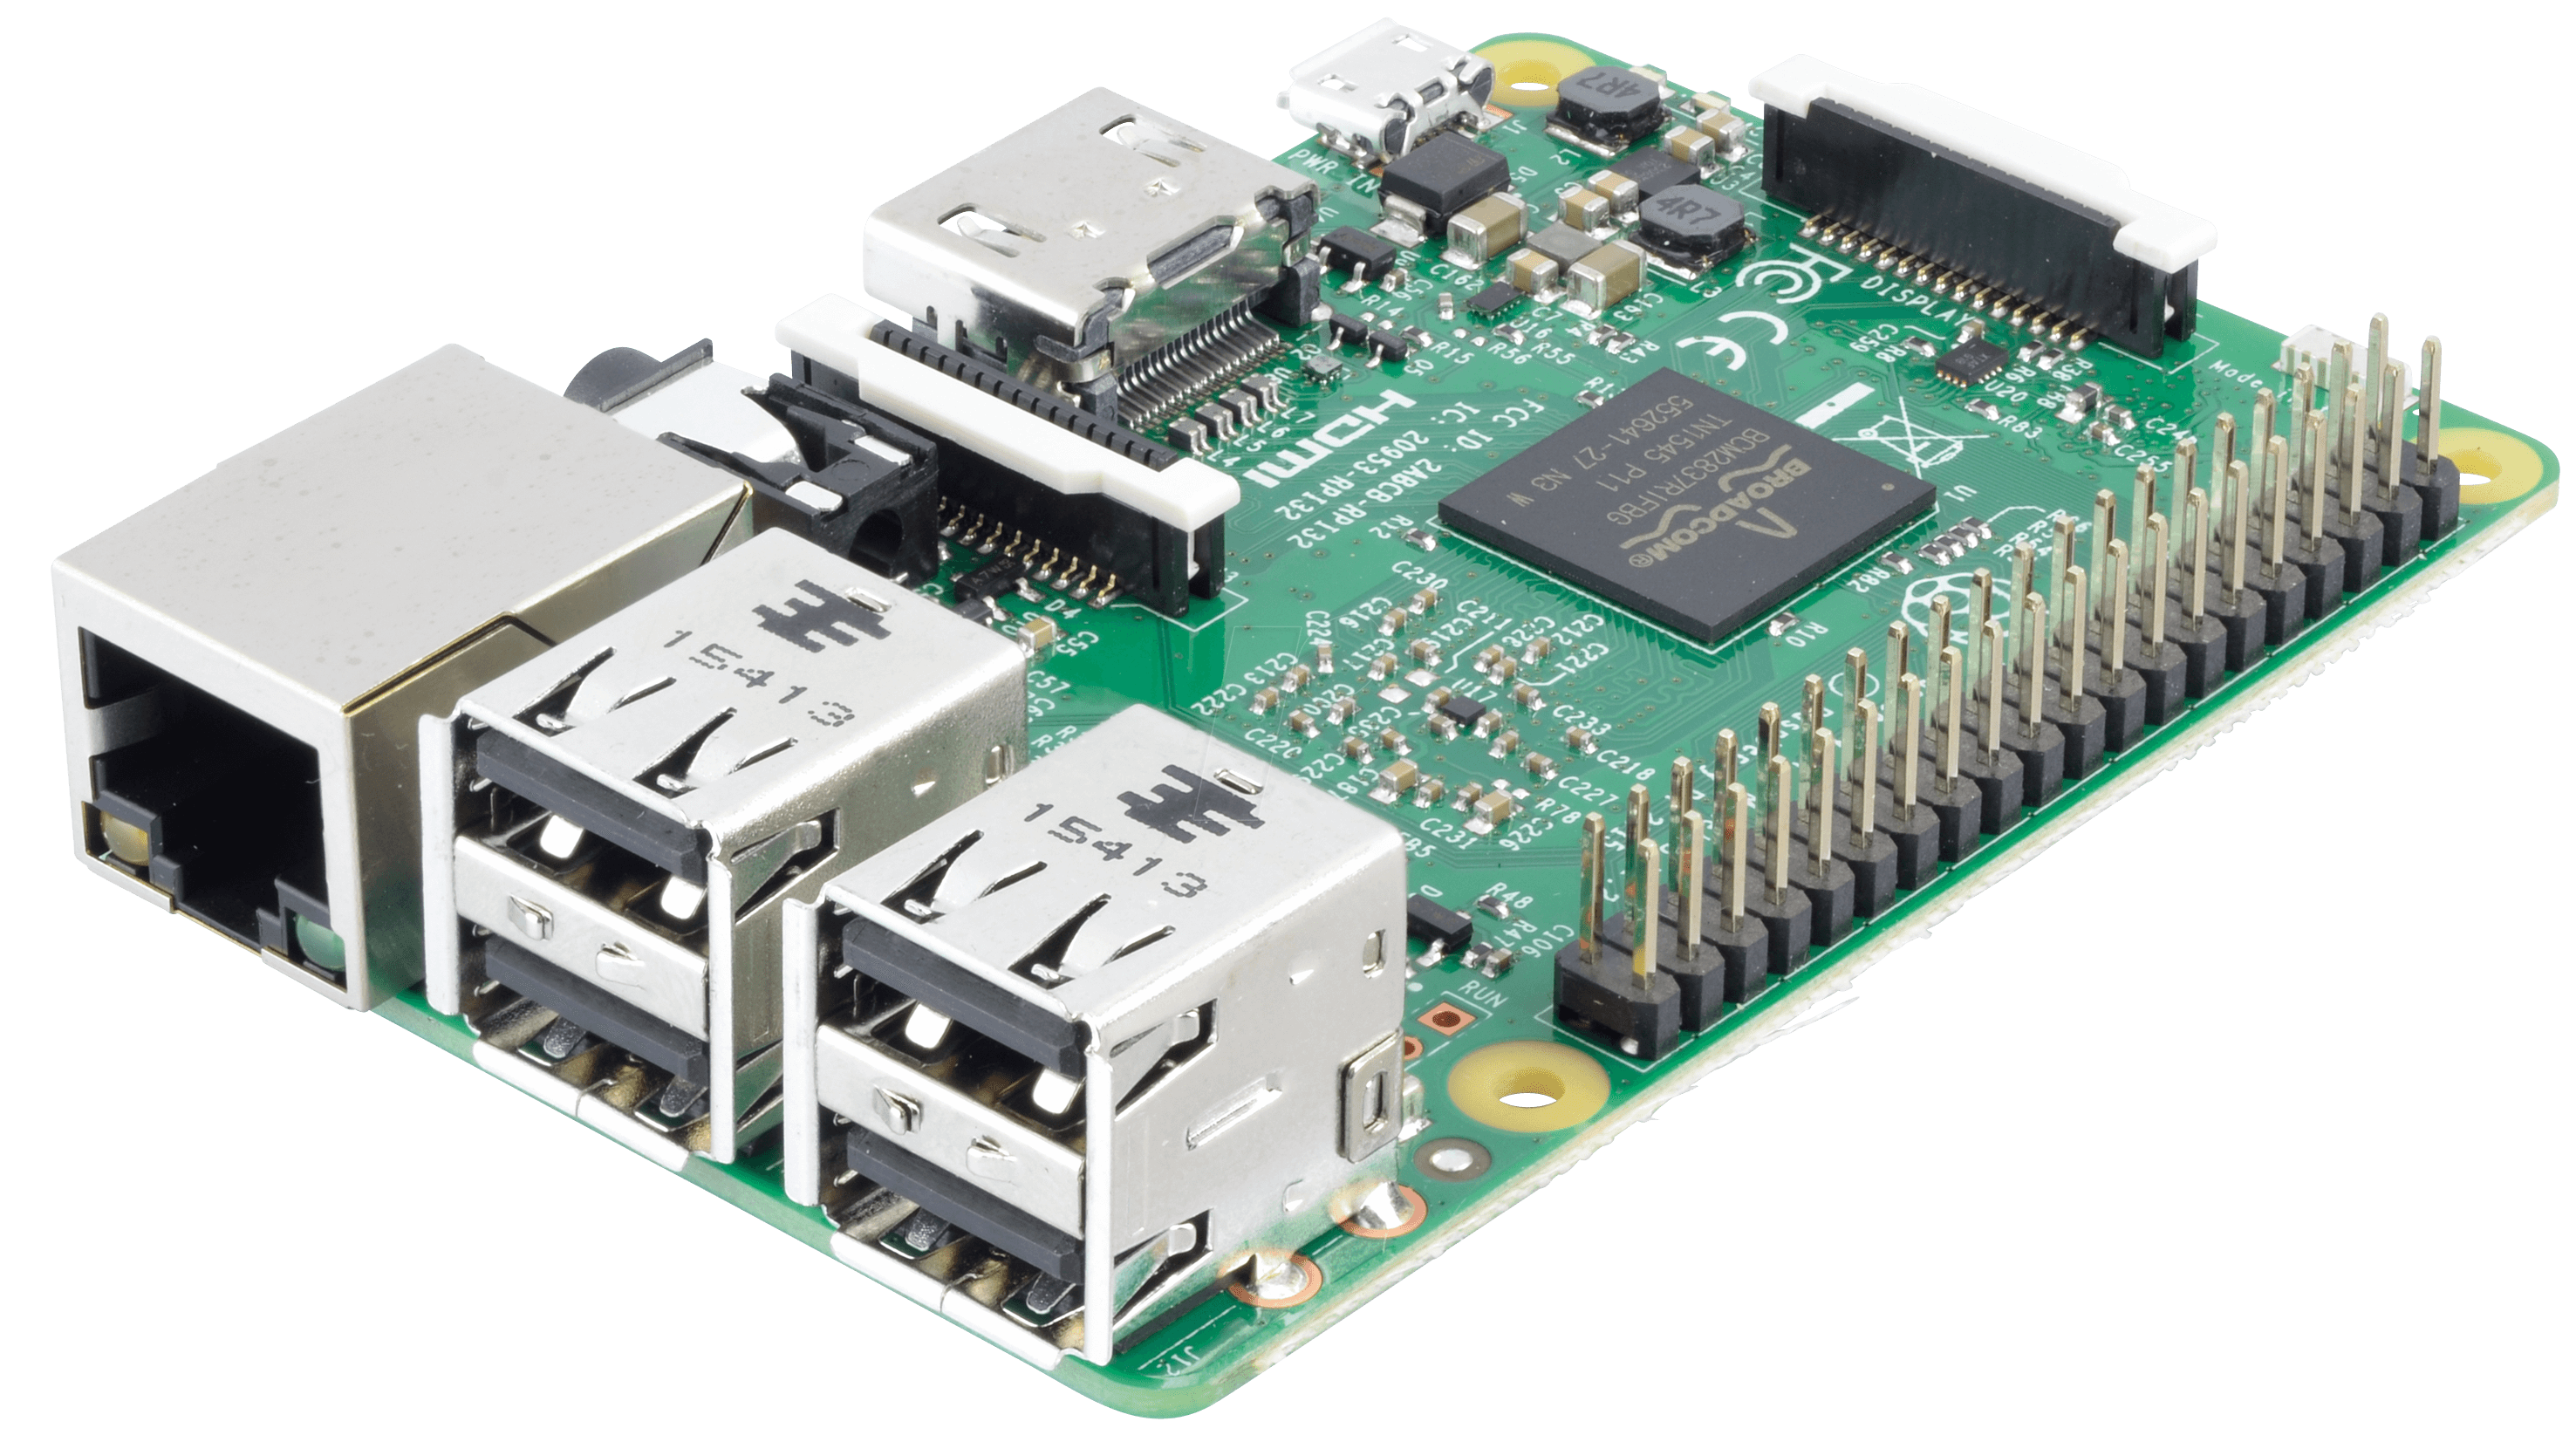
\includegraphics[width=.8\textwidth]{img/slide_rasp1.png}   
\end{center}
\end{column}
\begin{column}{0.3\textwidth}
\begin{center}
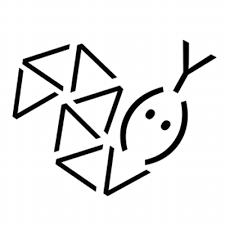
\includegraphics[width=.8\textwidth]{img/pythonanywhere_.png}    
\end{center}
\end{column}
\begin{column}{0.4\textwidth}
\begin{center}
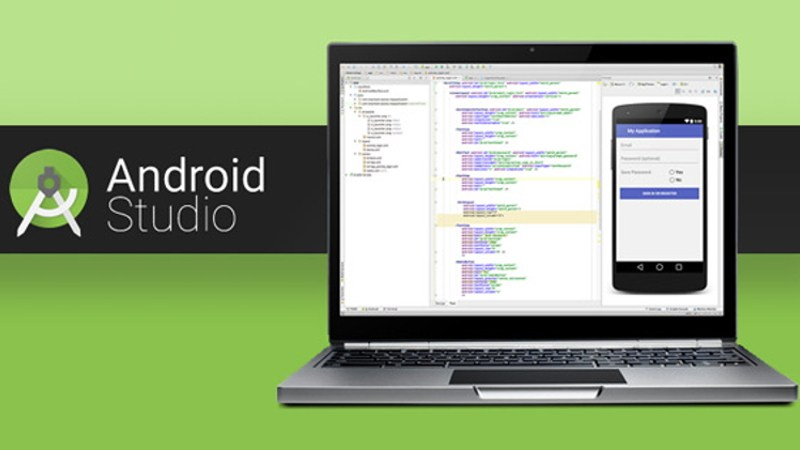
\includegraphics[width=.8\textwidth]{img/progr_android.jpg}    
\end{center}
\end{column}
\end{columns}
\begin{columns}
\begin{column}{0.6\textwidth}
\begin{center}

\includegraphics[width=.7\textwidth]{img/progr_python.png}   
\end{center}
\end{column}
\begin{column}{0.4\textwidth}
\begin{center}

\includegraphics[width=.8\textwidth]{img/progr_java.png}    
\end{center}
\end{column}
\end{columns}
\end{frame}


\subsection{Arquitetura do Projeto}

\begin{frame}{Arquitetura do Projeto}


\begin{center}
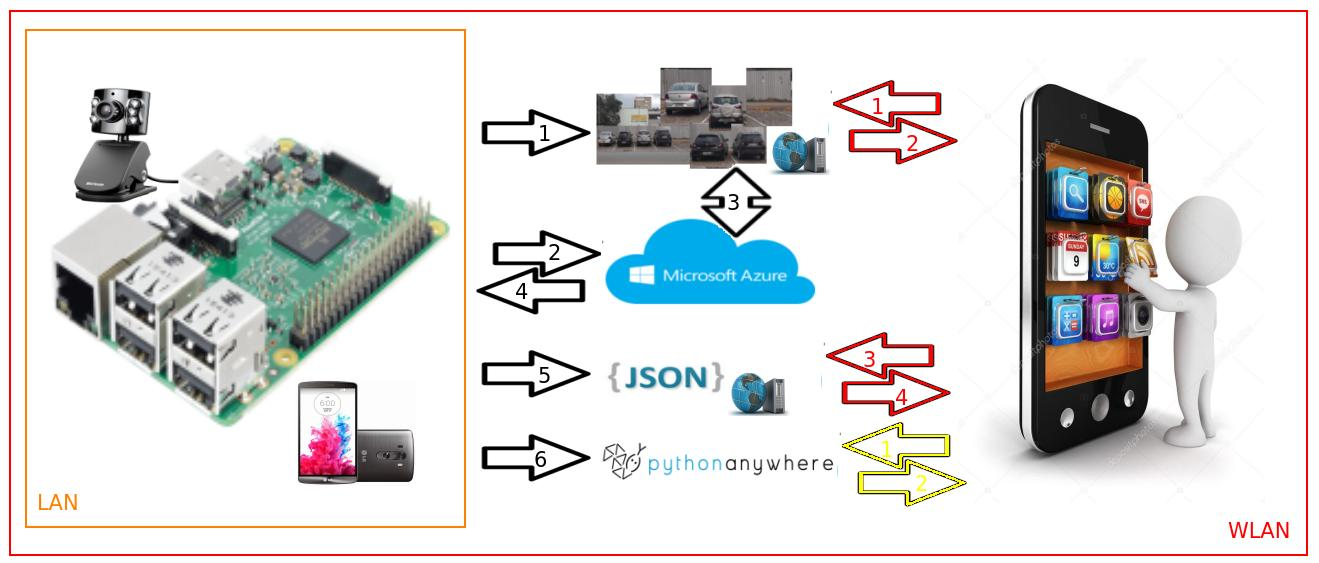
\includegraphics[width=1\textwidth]{img/estrutura.jpeg}   
\end{center}

\end{frame}



\subsection{Experimentos }

\begin{frame}{Experimentos}
Funcionamento do API Computer Vision

\begin{center}
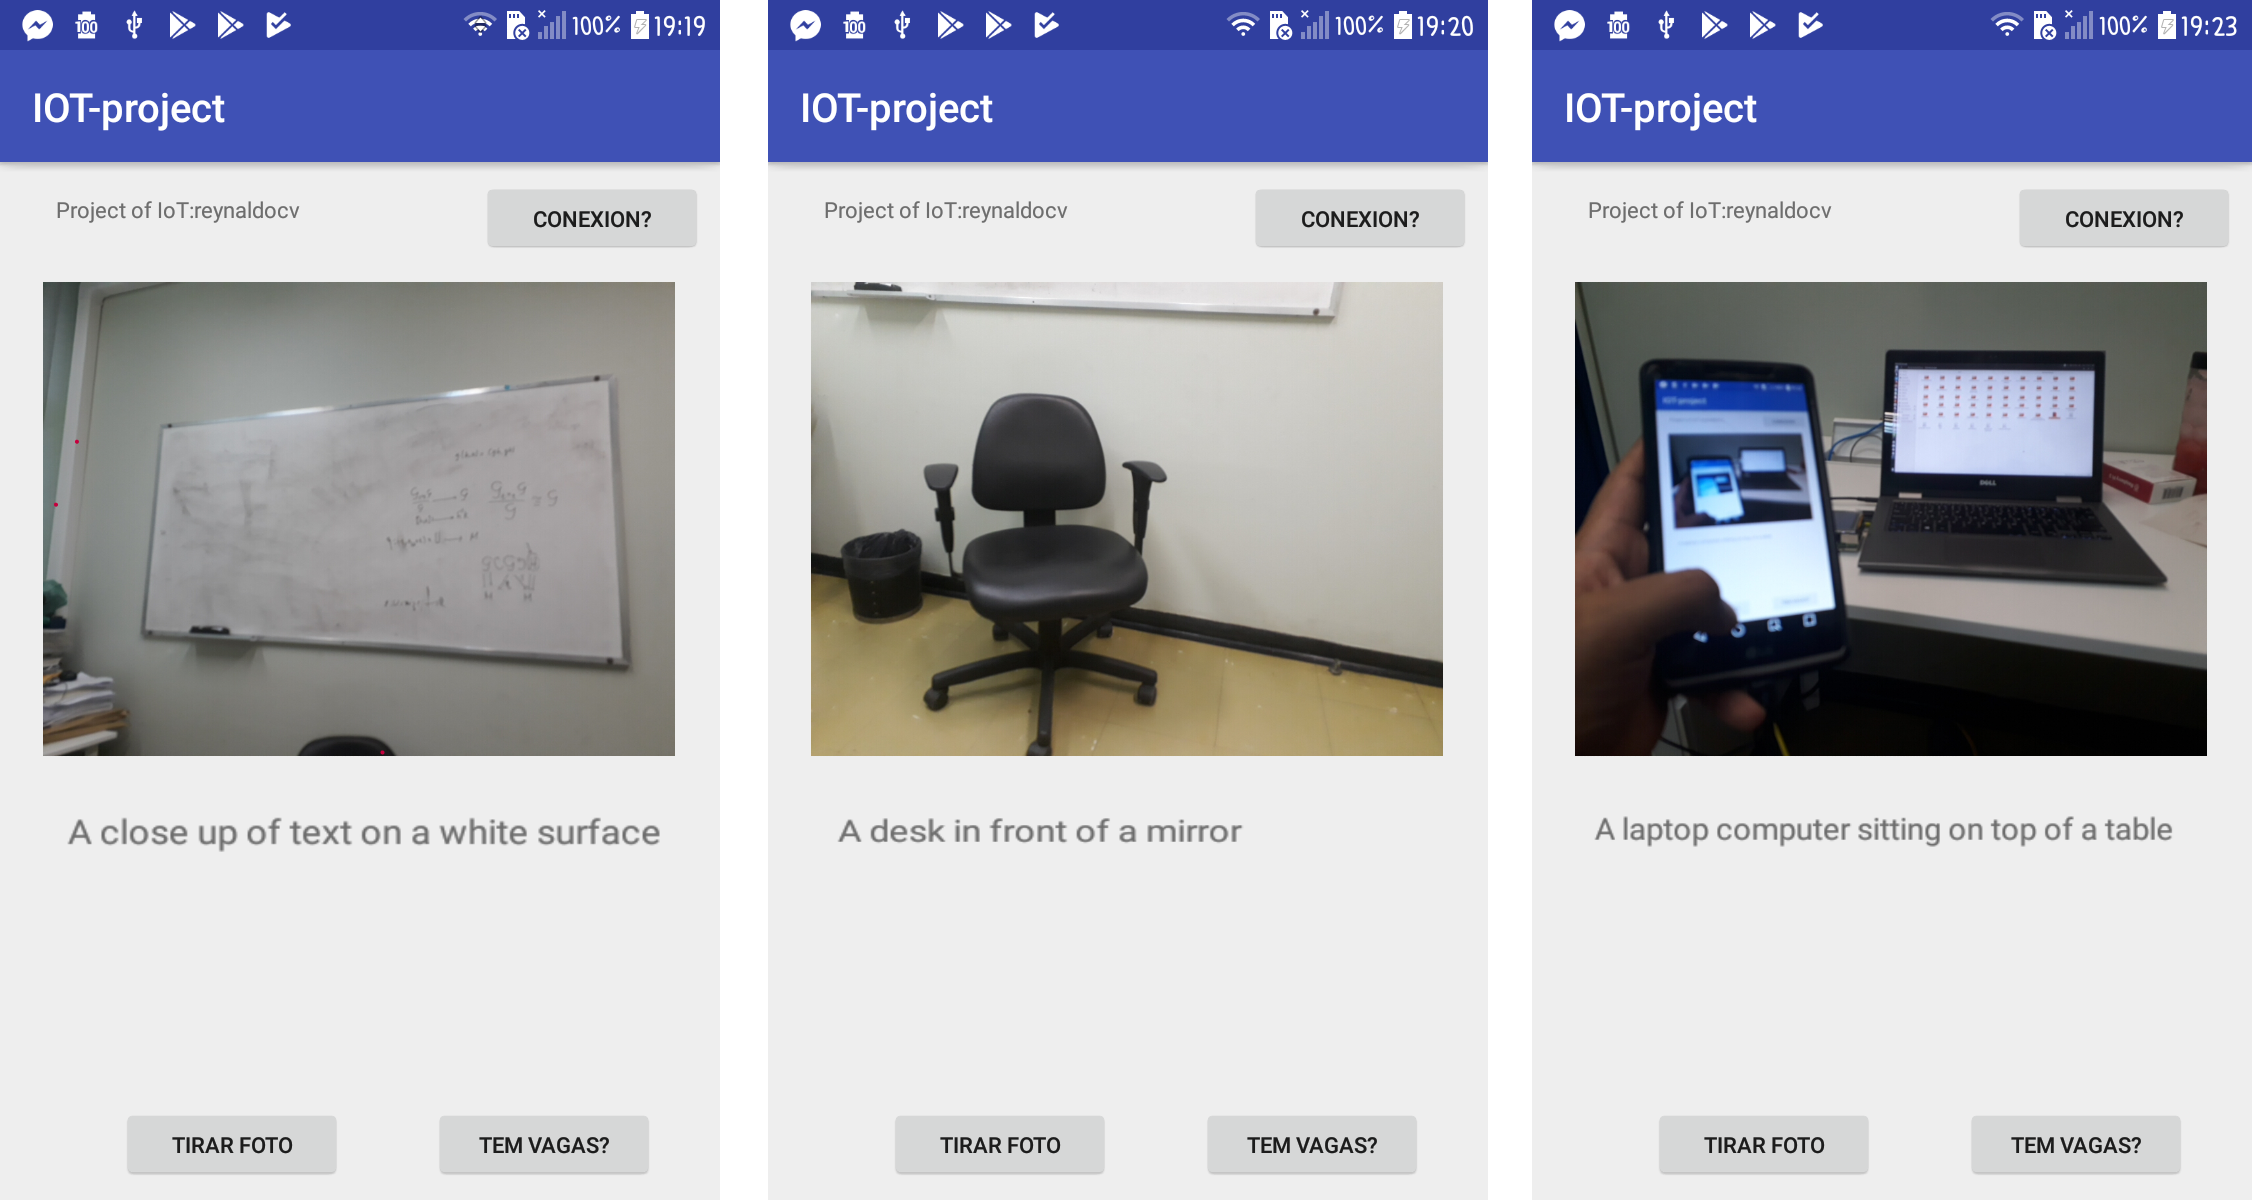
\includegraphics[width=.9\textwidth]{img/app_1.png}   
\end{center}
\begin{itemize}\tiny
 \item Conexão direta entre o Raspberry e o Celular (mesma LAN)  
\end{itemize}

\end{frame}

\begin{frame}{Experimentos}
Funcionamento do API Computer Vision

\begin{center}
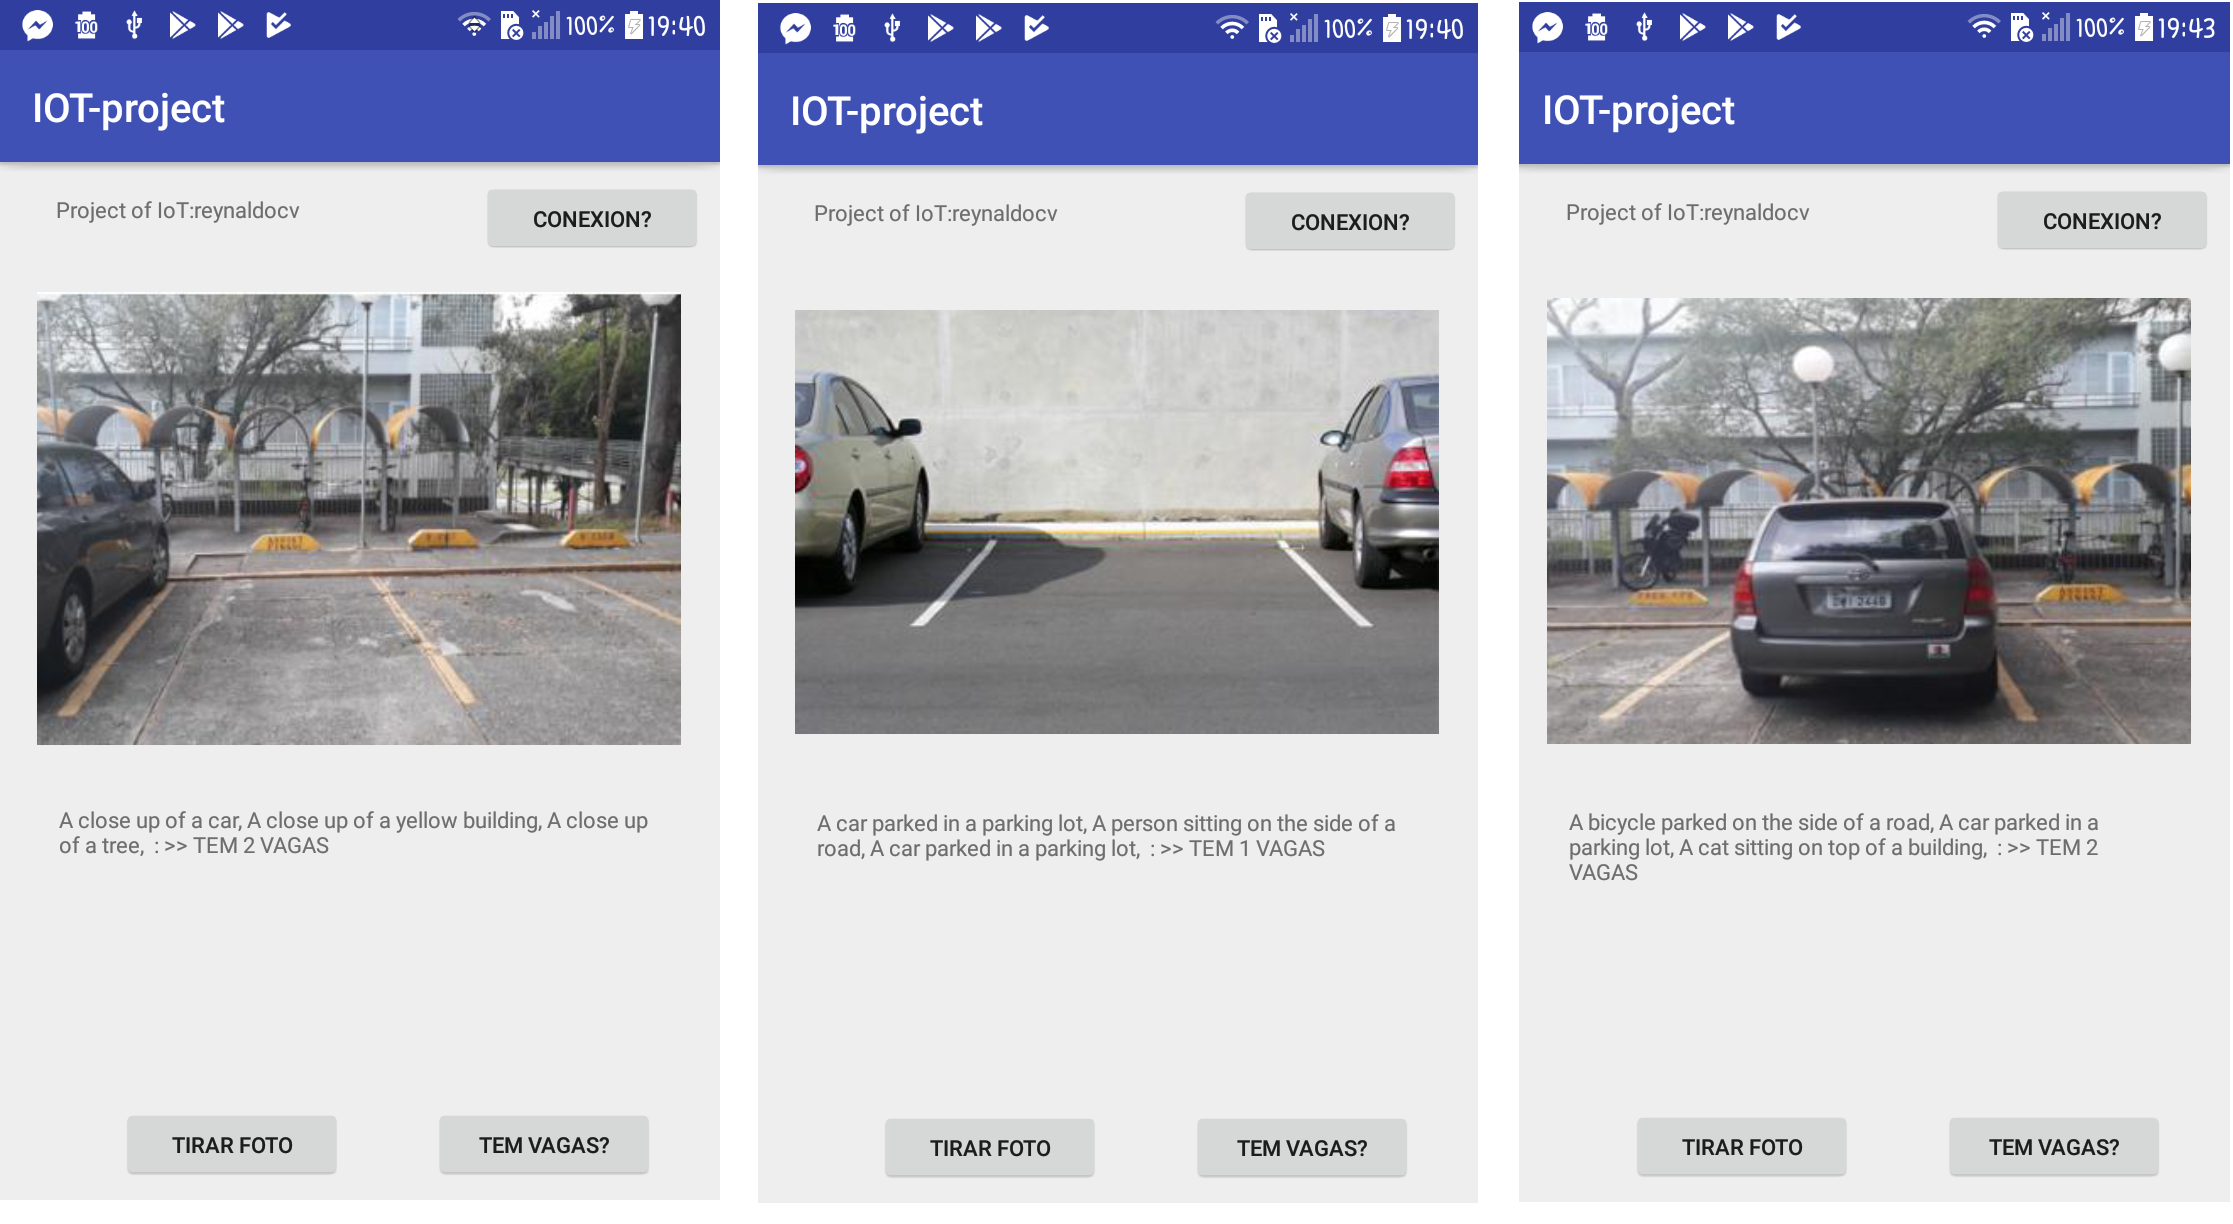
\includegraphics[width=.9\textwidth]{img/app_2.png}   
\end{center}
\begin{itemize}\tiny
 \item Conexão direta entre o Raspberry e o Celular (mesma LAN)  
\end{itemize}

\end{frame}



\begin{frame}{Experimentos}
Funcionamento com carrinhos

\begin{center}
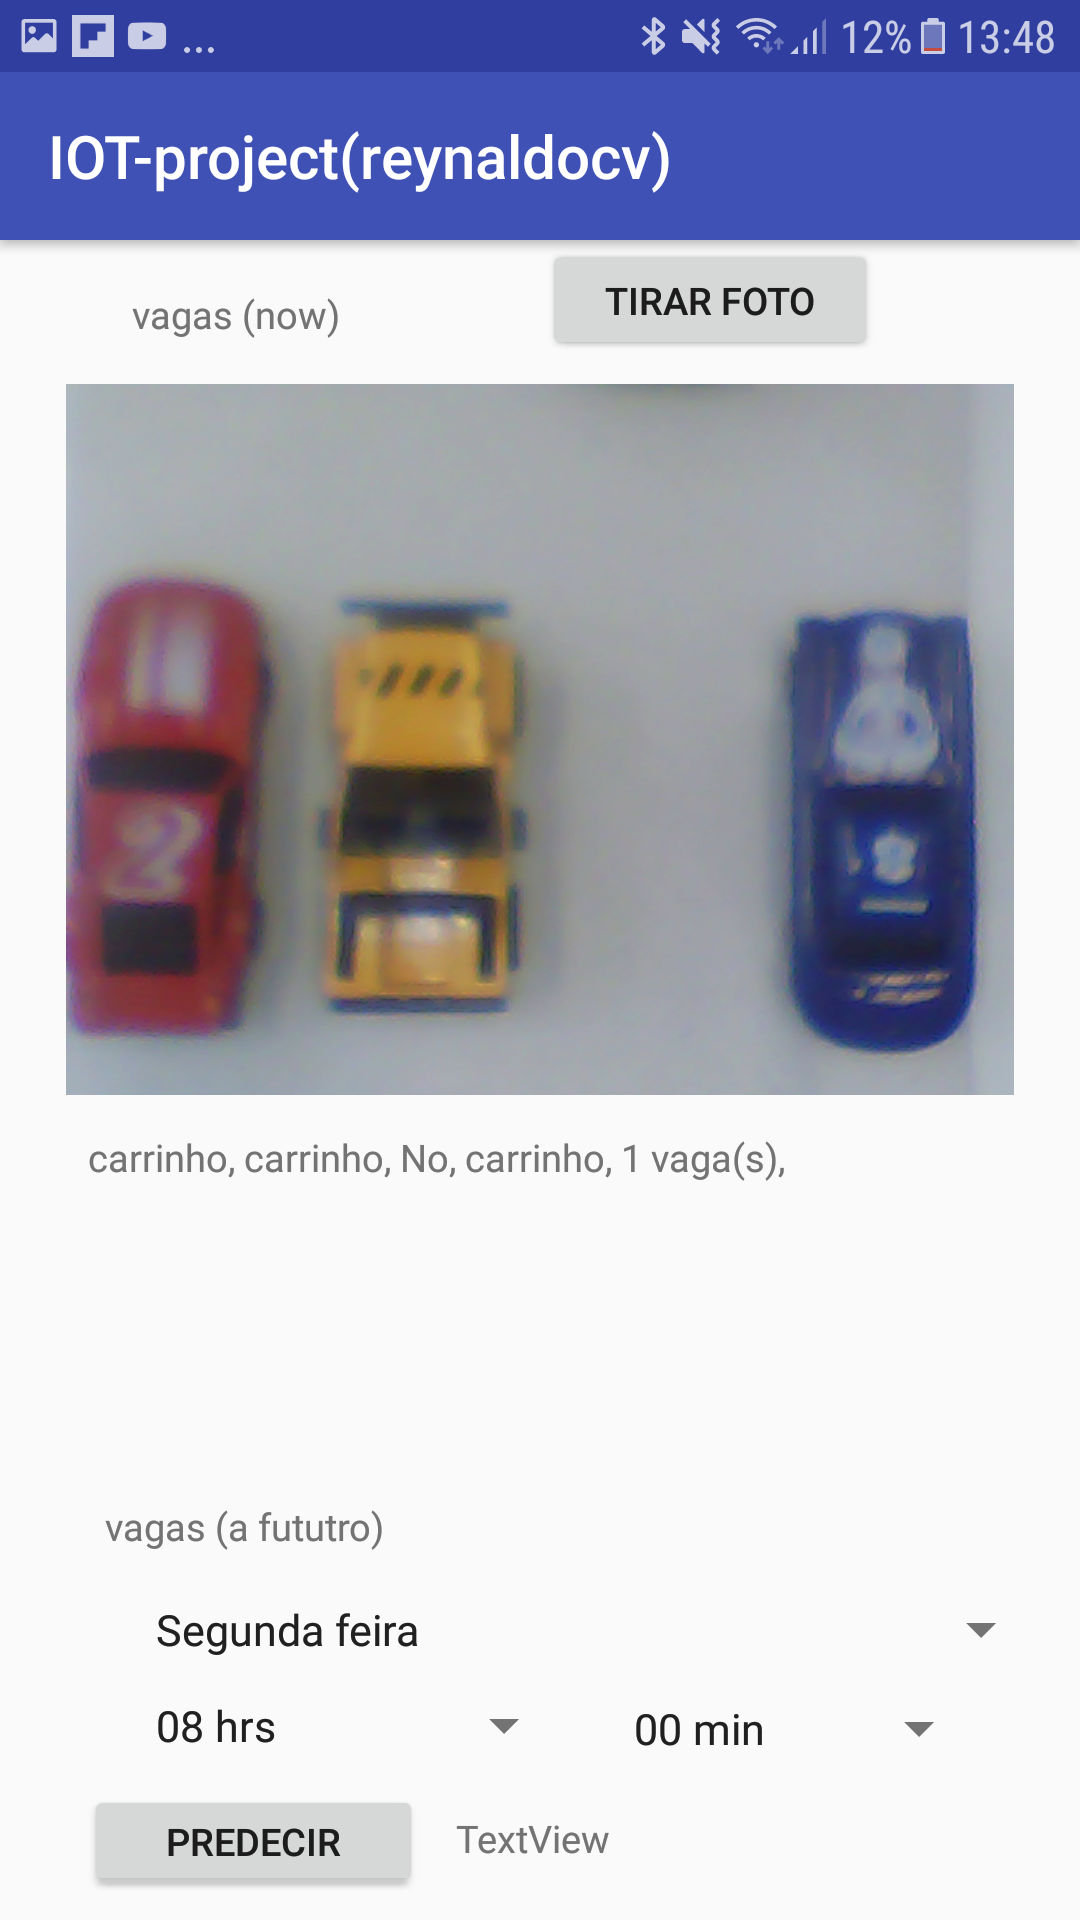
\includegraphics[width=.3\textwidth]{img/carrinho_1.png}\ \ 
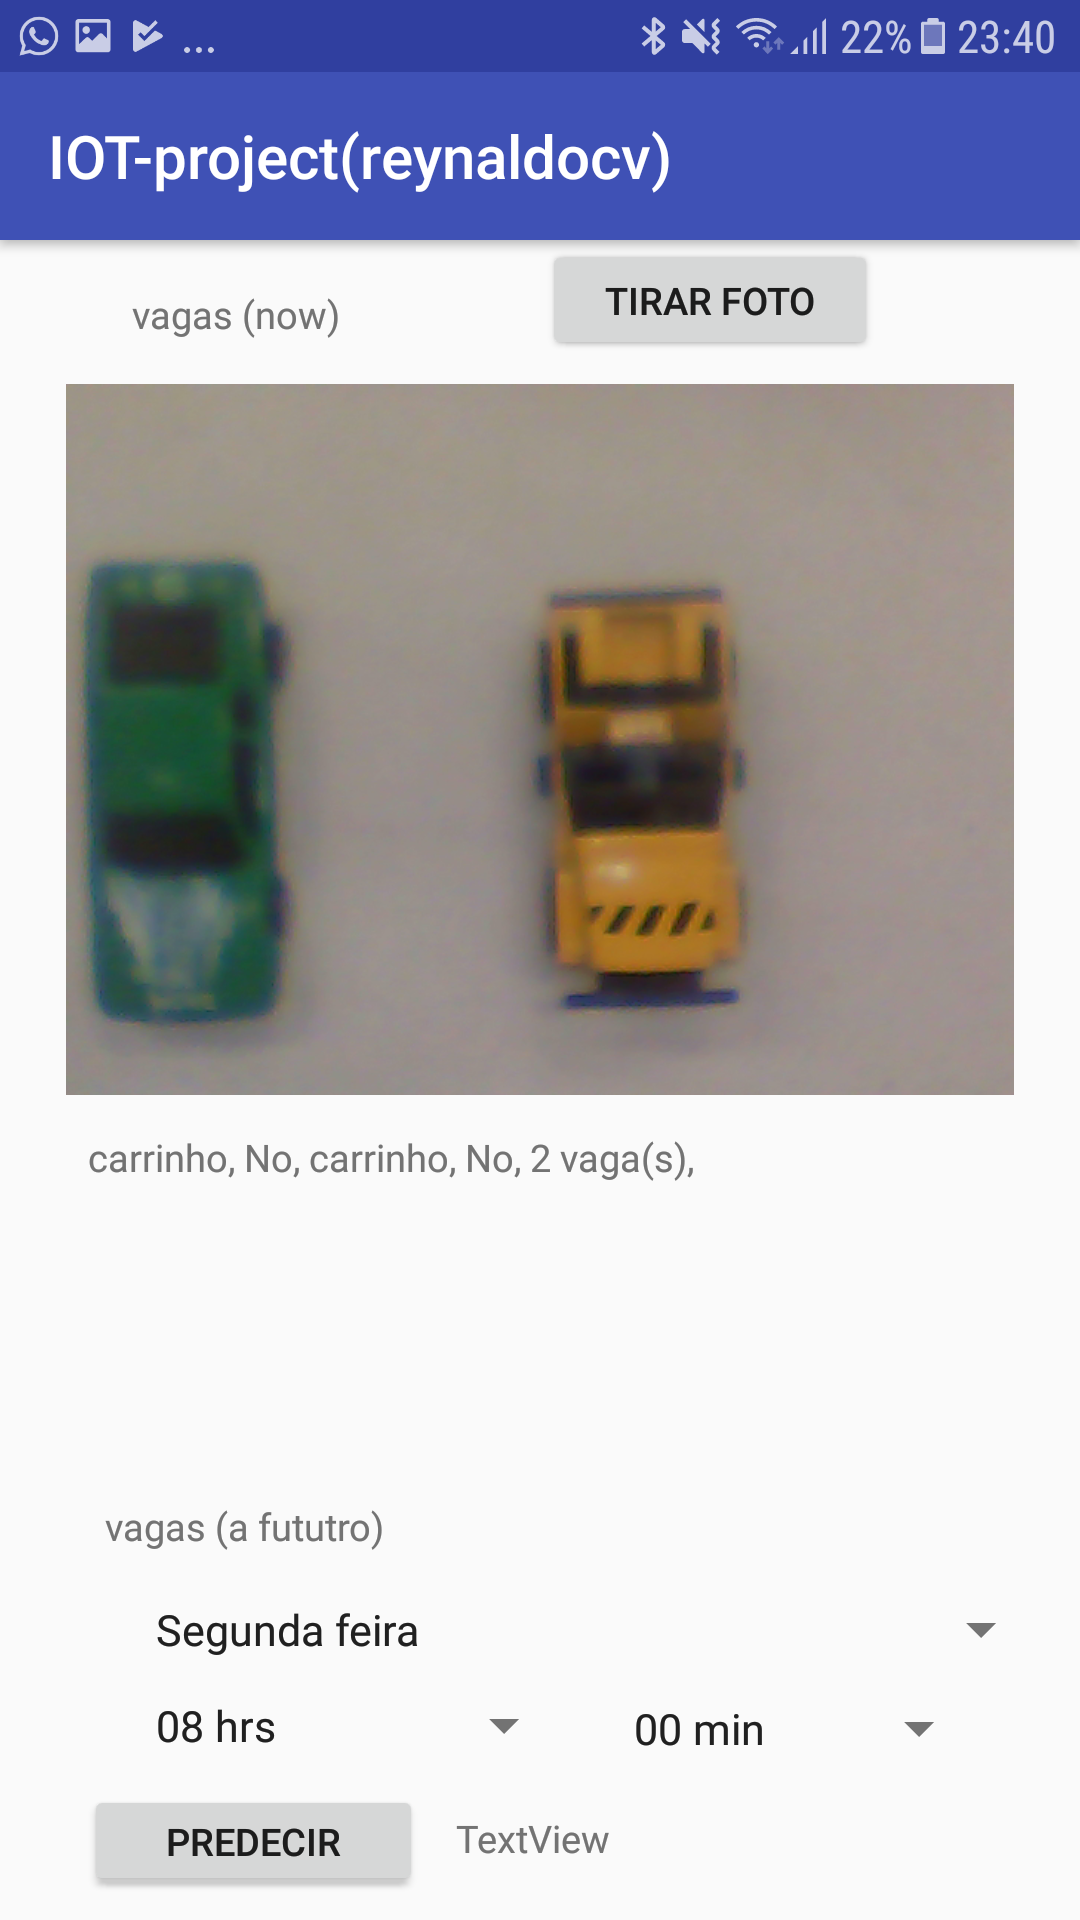
\includegraphics[width=.3\textwidth]{img/carrinho_2.png}\ \   
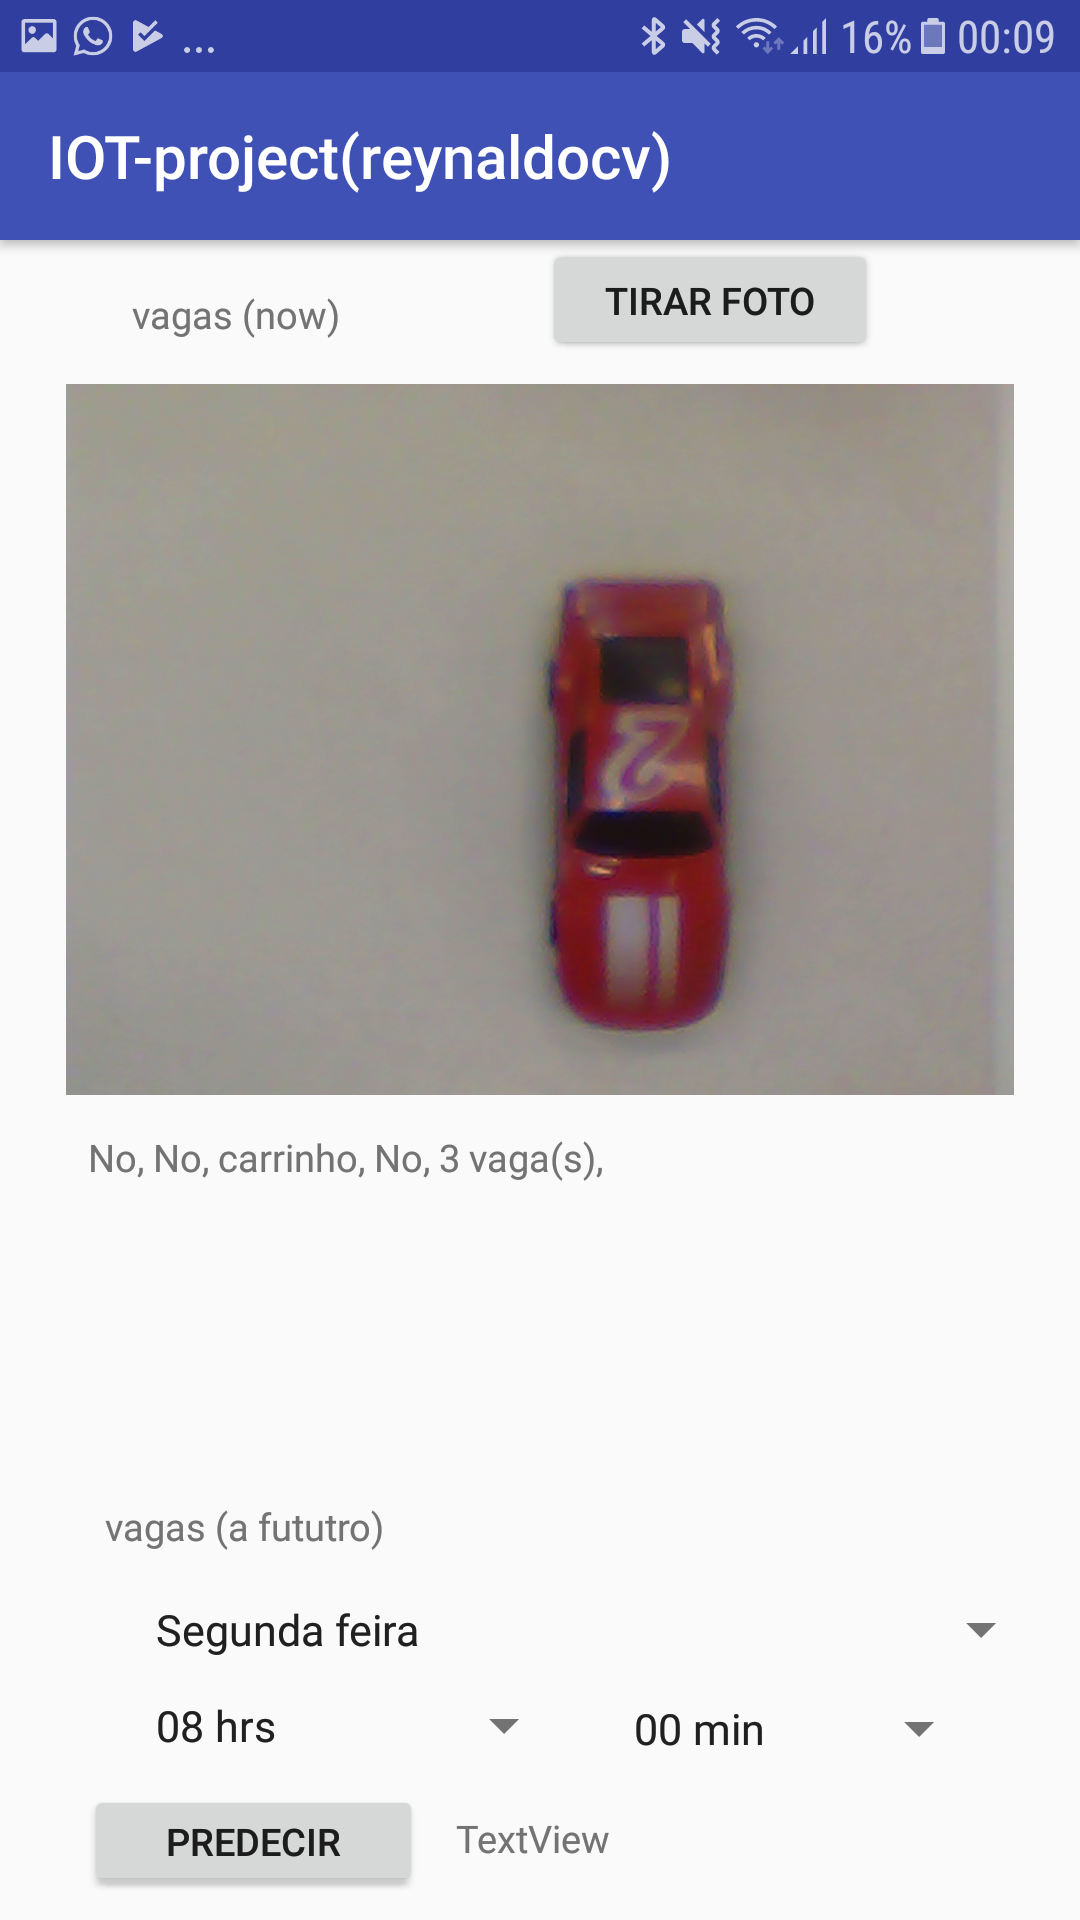
\includegraphics[width=.3\textwidth]{img/carrinho_3.png}   
\end{center}
\end{frame}

\begin{frame}{Experimentos}
Funcionamento com carrinhos

\begin{center}
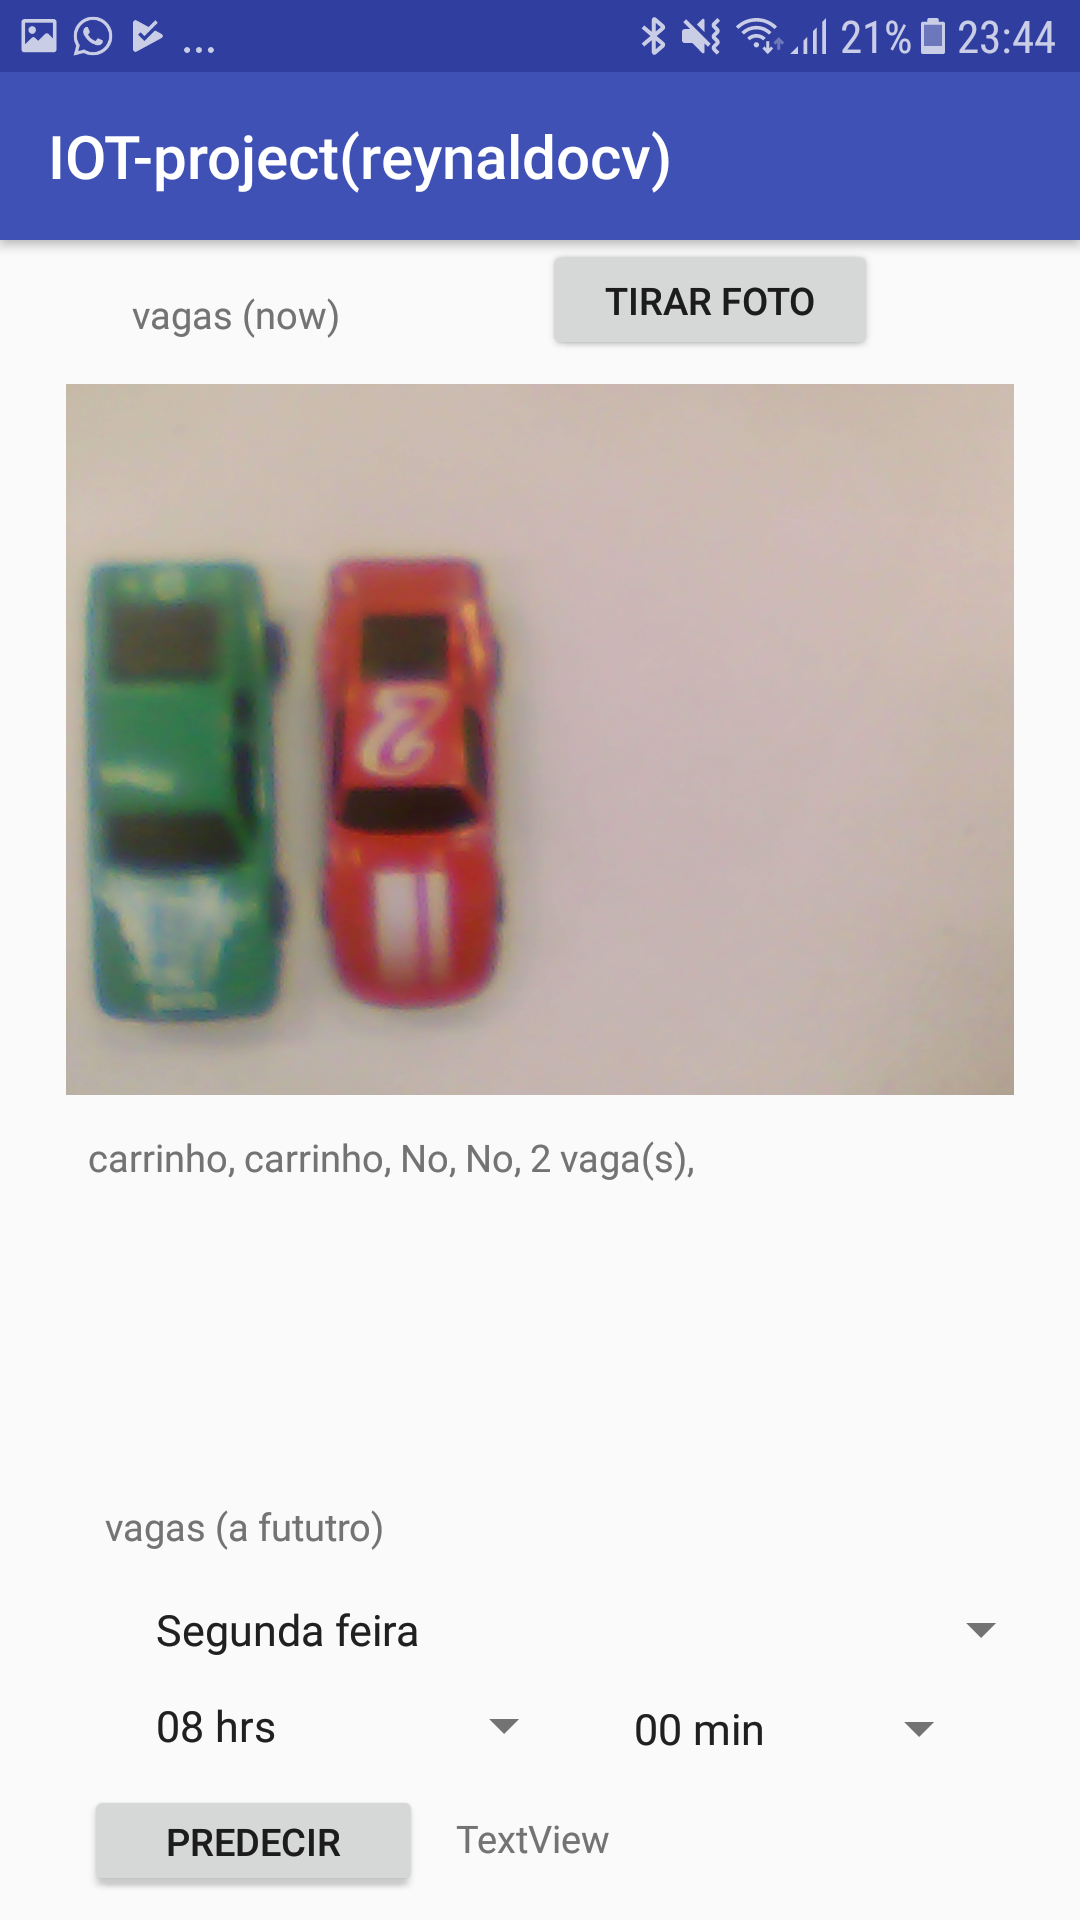
\includegraphics[width=.3\textwidth]{img/carrinho_4.png}\ \ 
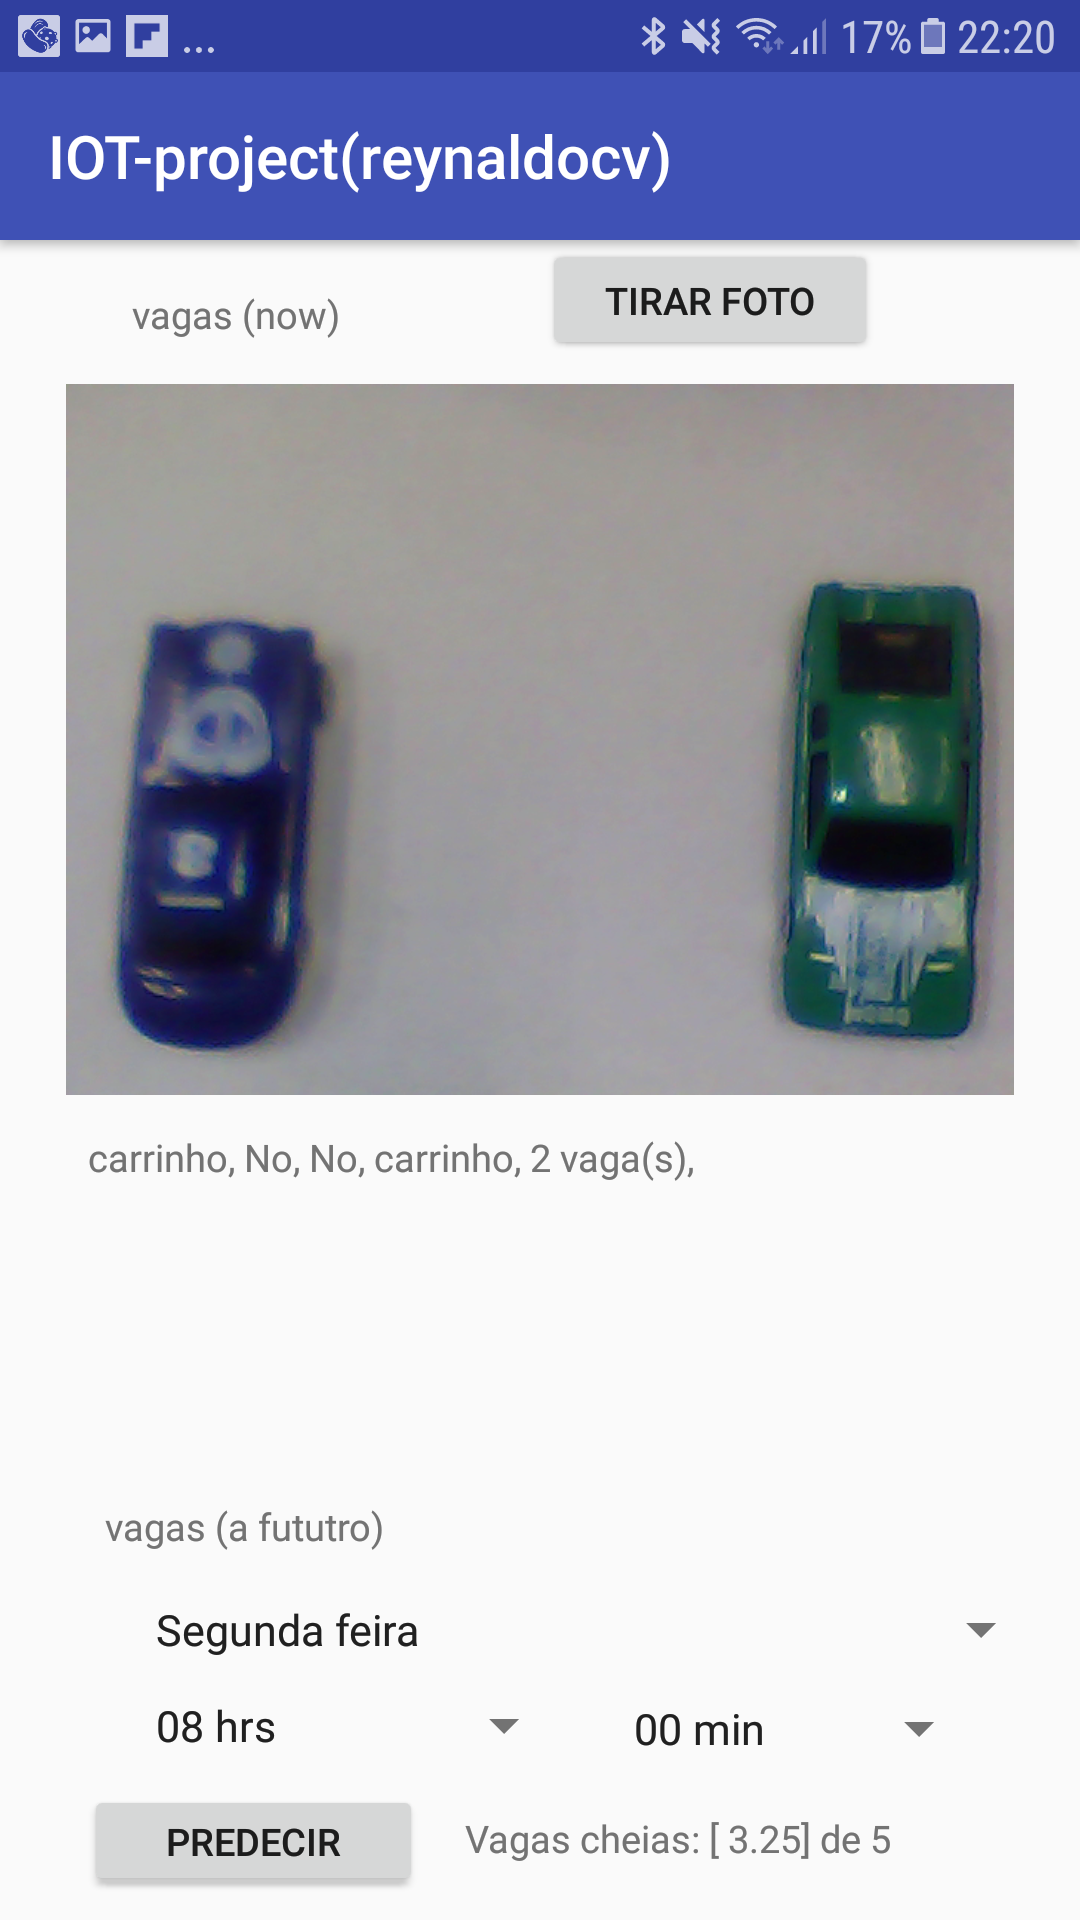
\includegraphics[width=.3\textwidth]{img/carrinho_5.png}\ \   
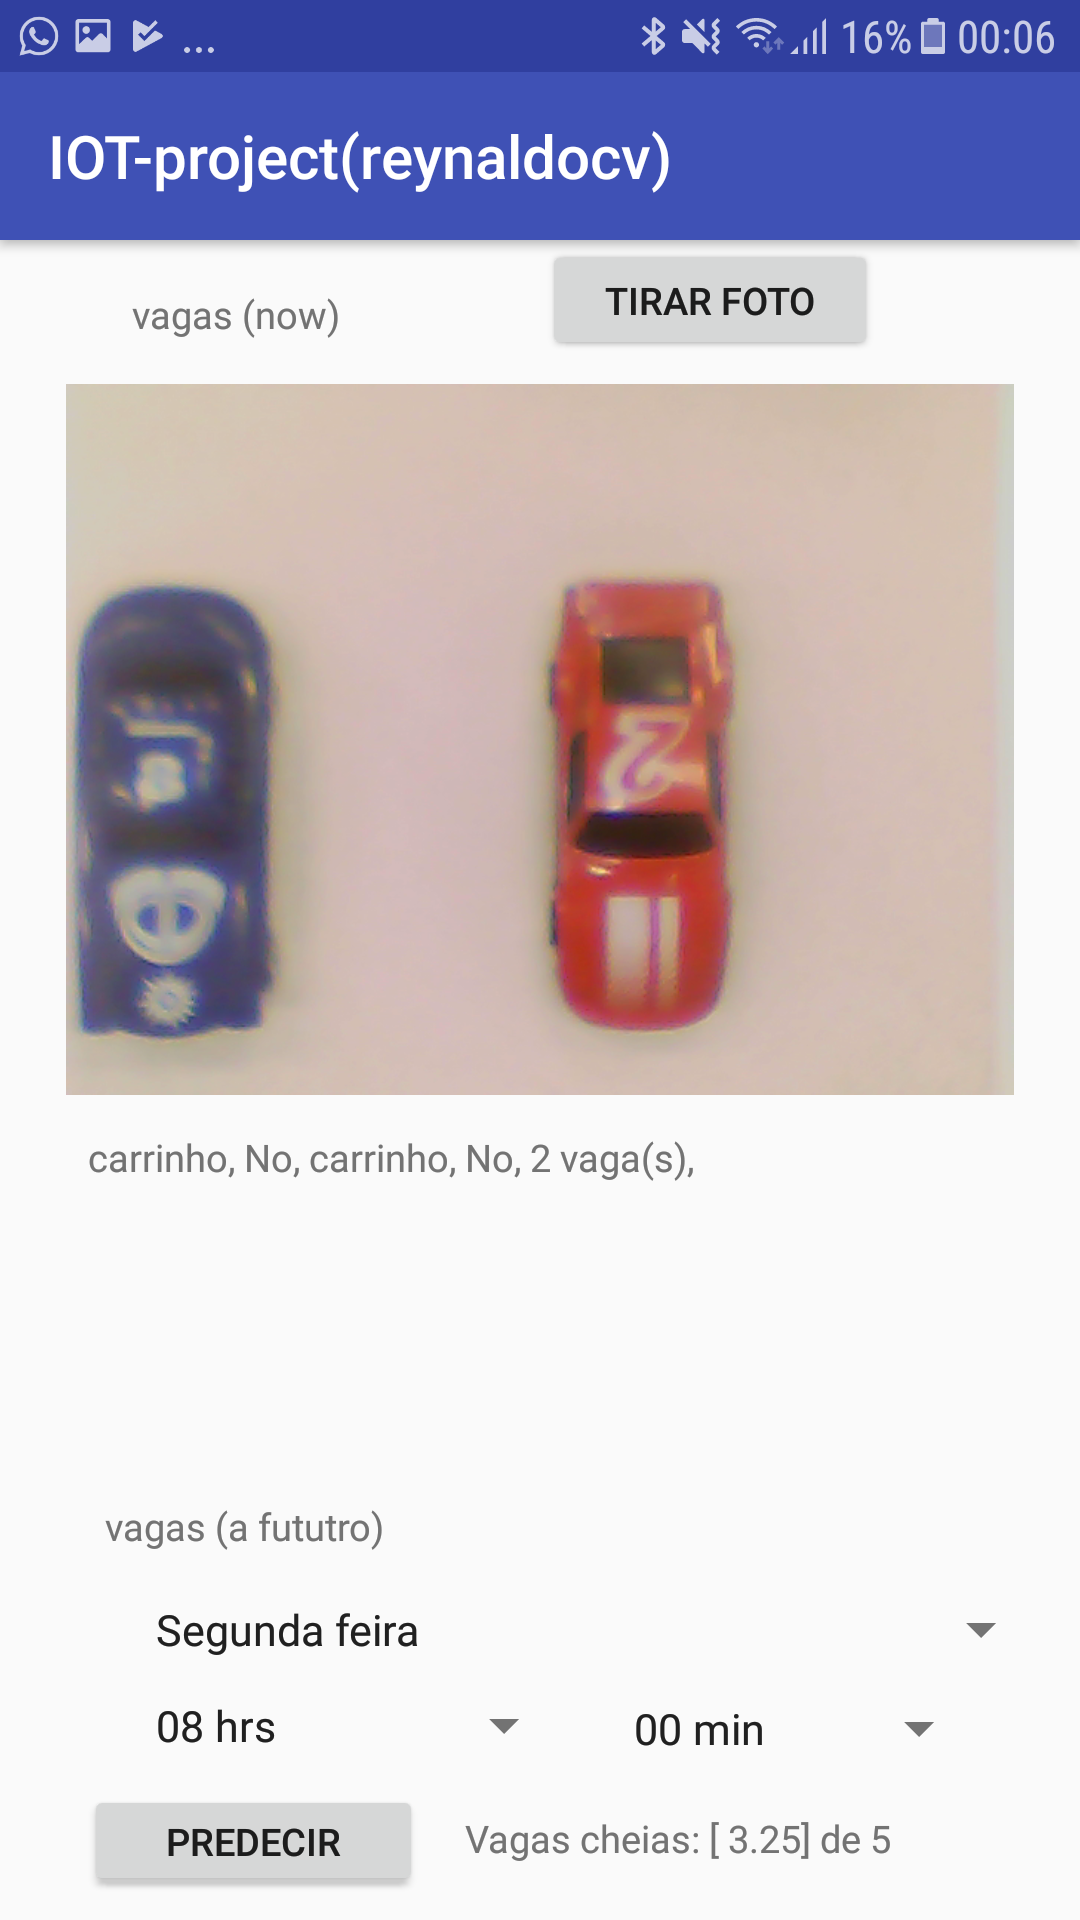
\includegraphics[width=.3\textwidth]{img/carrinho_6.png}   
\end{center}
\end{frame}


\begin{frame}{Experimentos}
Funcionamento

\begin{center}
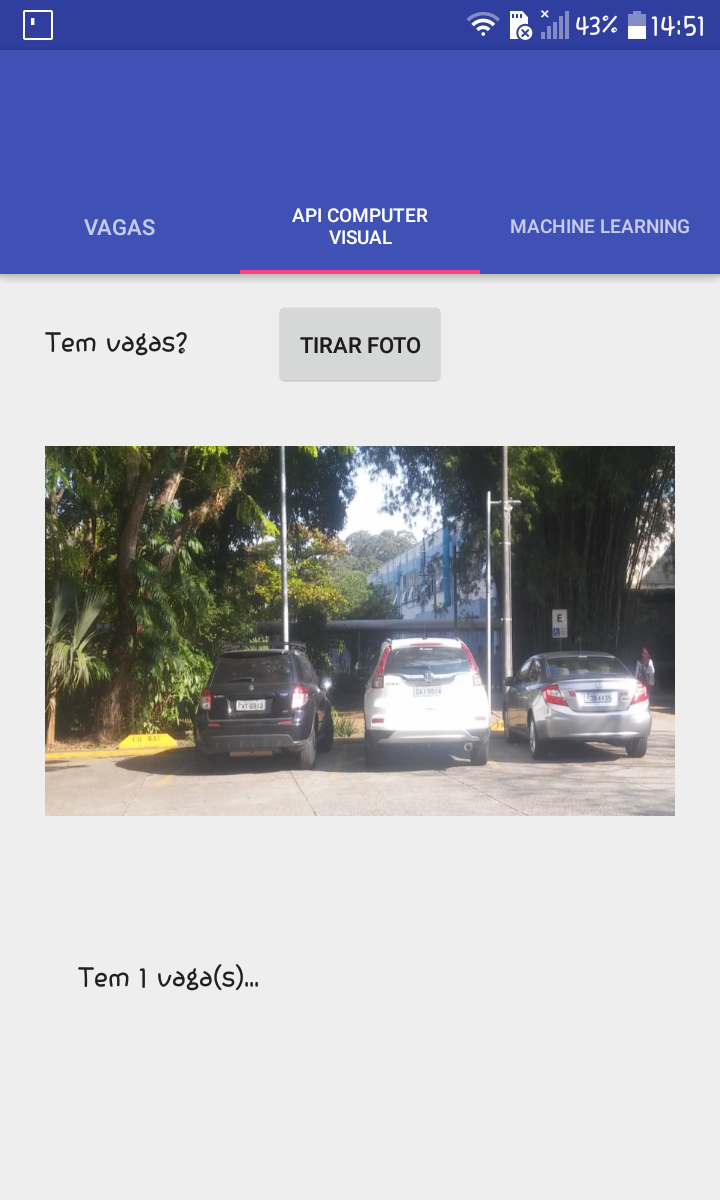
\includegraphics[width=.3\textwidth]{img/app_foto_1.png}\ \ \ \ \   
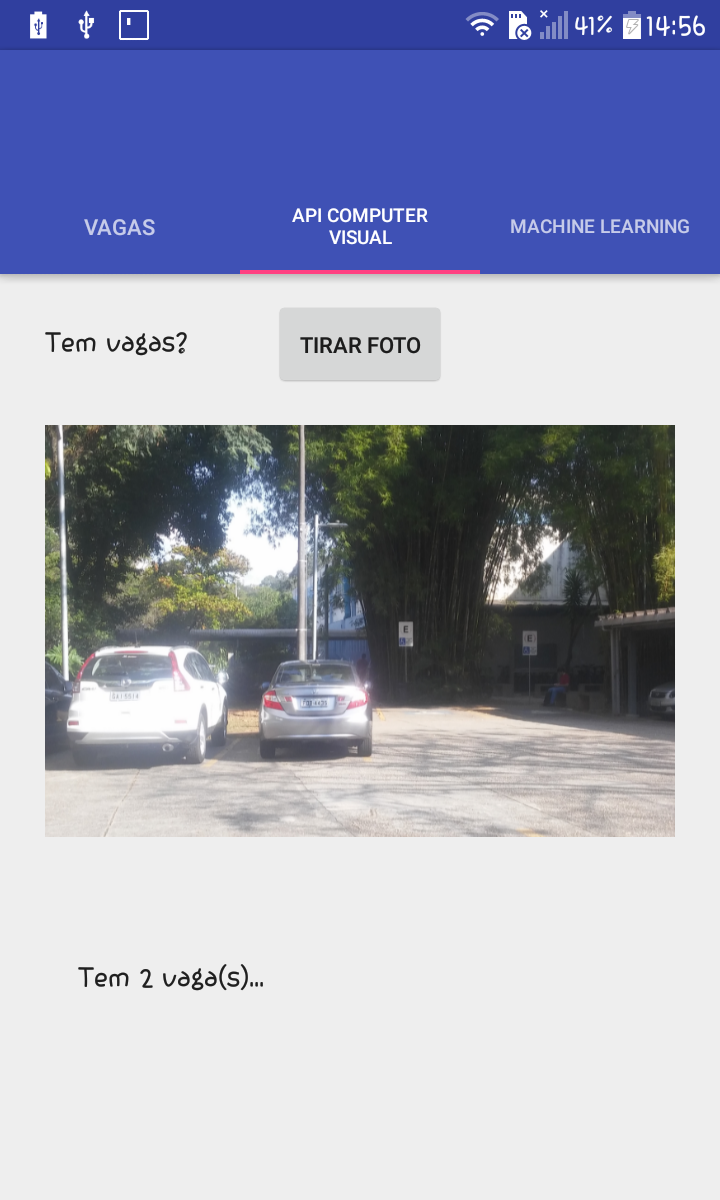
\includegraphics[width=.3\textwidth]{img/app_foto_2.png}   
\end{center}

\end{frame}





\subsubsection{Aplicação de Machine Learning}

\begin{frame}{Aplicação de Machine Learning}
APIs criadas no pythonanywhere:
\begin{itemize}\tiny
 \item $http://reynaldocv.pythonanywhere.com/add/<text1>$
 \item $http://reynaldocv.pythonanywhere.com/dataset$
 
 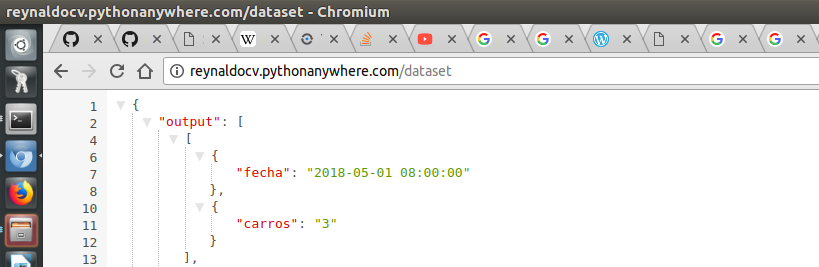
\includegraphics[width=.8\textwidth]{img/paw_dataset.png}
 
 \item $http://reynaldocv.pythonanywhere.com/futuro/<dia>/<hora>/<minutos>$
 
 
 Biblioteca sklearn, e o algoritmo Decision-Tree-Regressor (Acurácia de 67\%)
 
 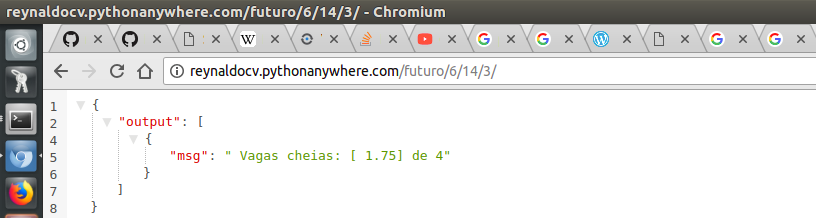
\includegraphics[width=.8\textwidth]{img/paw_futuro.png}
 
 
\end{itemize}
\end{frame}



\begin{frame}{Experimentos(Junho- 2018)}
Consulta de vagas no futuro:

\begin{center}
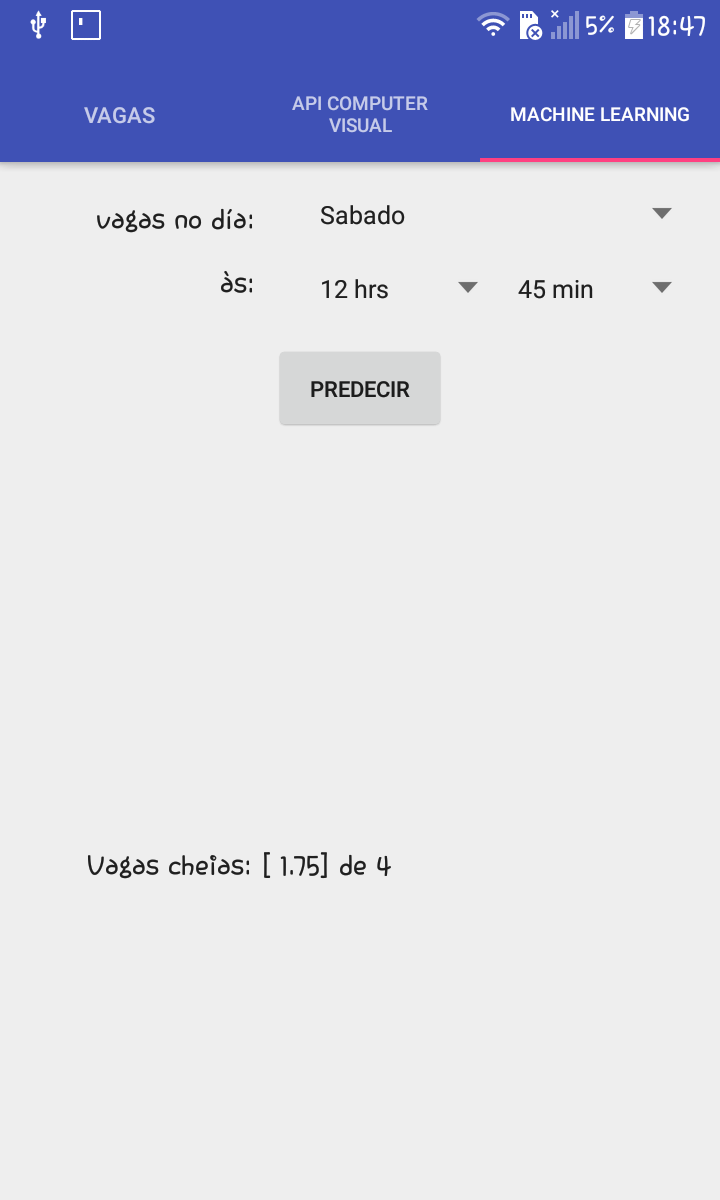
\includegraphics[width=.3\textwidth]{img/futuro_1.png}\ \ 
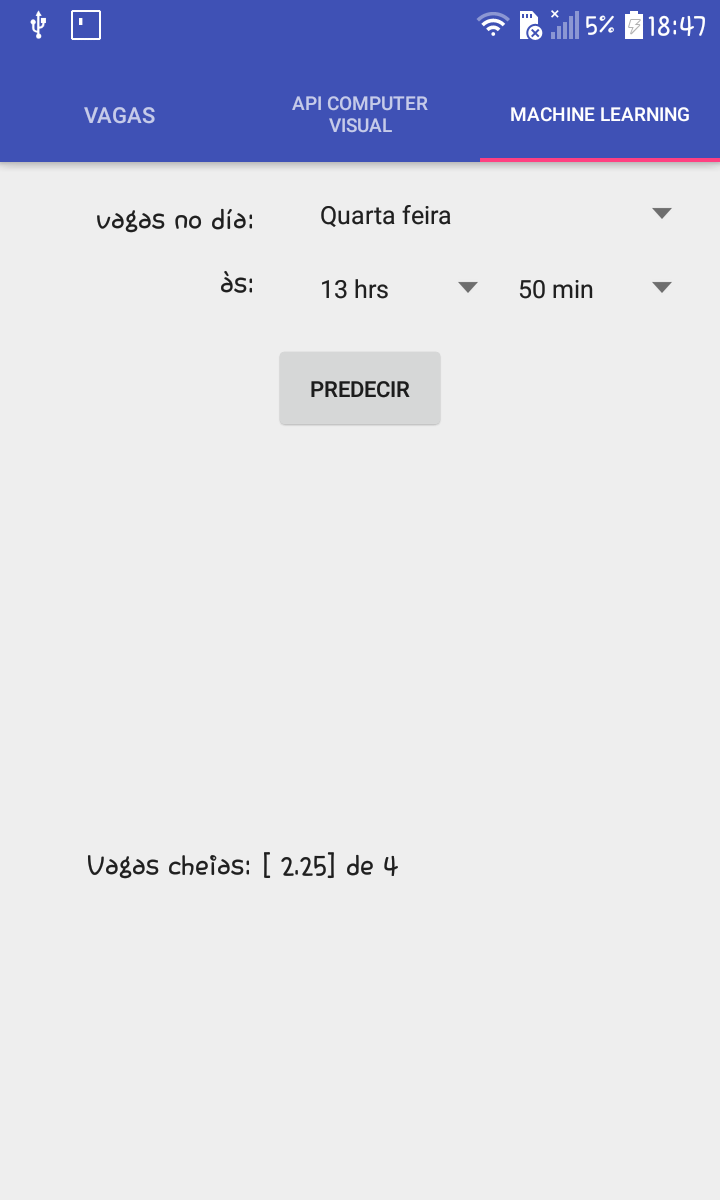
\includegraphics[width=.3\textwidth]{img/futuro_2.png}\ \   
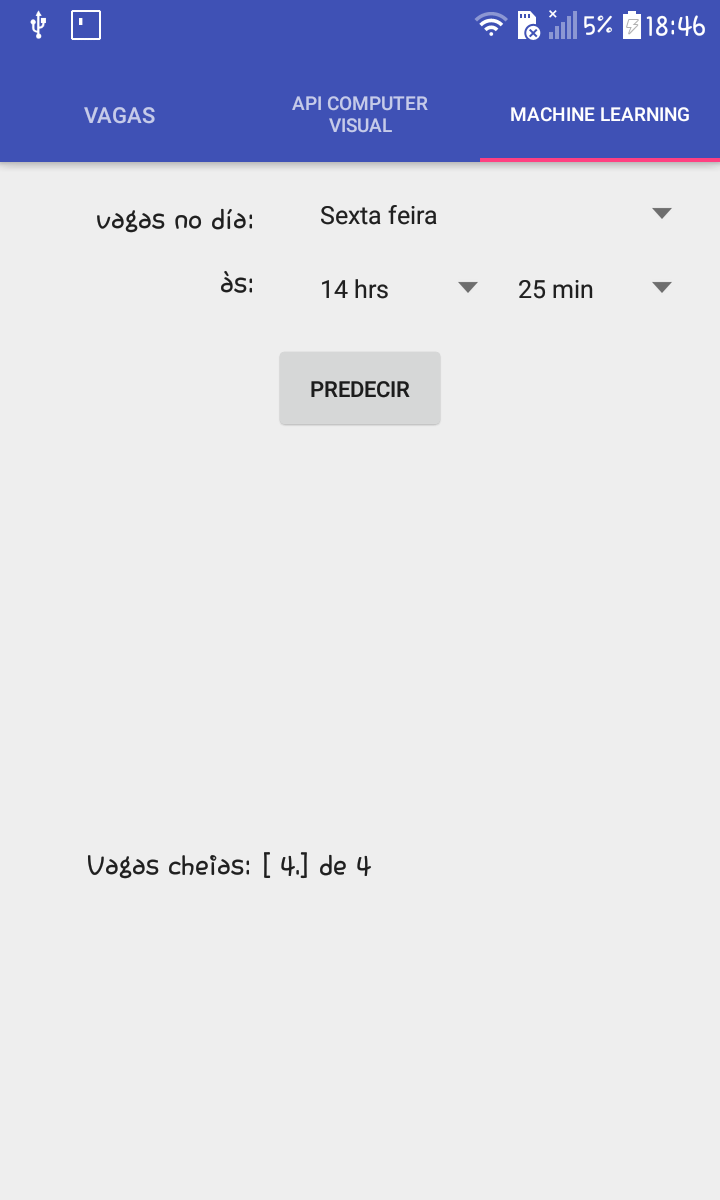
\includegraphics[width=.3\textwidth]{img/futuro_3.png}   
\end{center}
\end{frame}

\begin{frame}{}
  \tableofcontents
\end{frame}

\section{Conclusões}


\begin{frame}{Conclusões}
\begin{center}
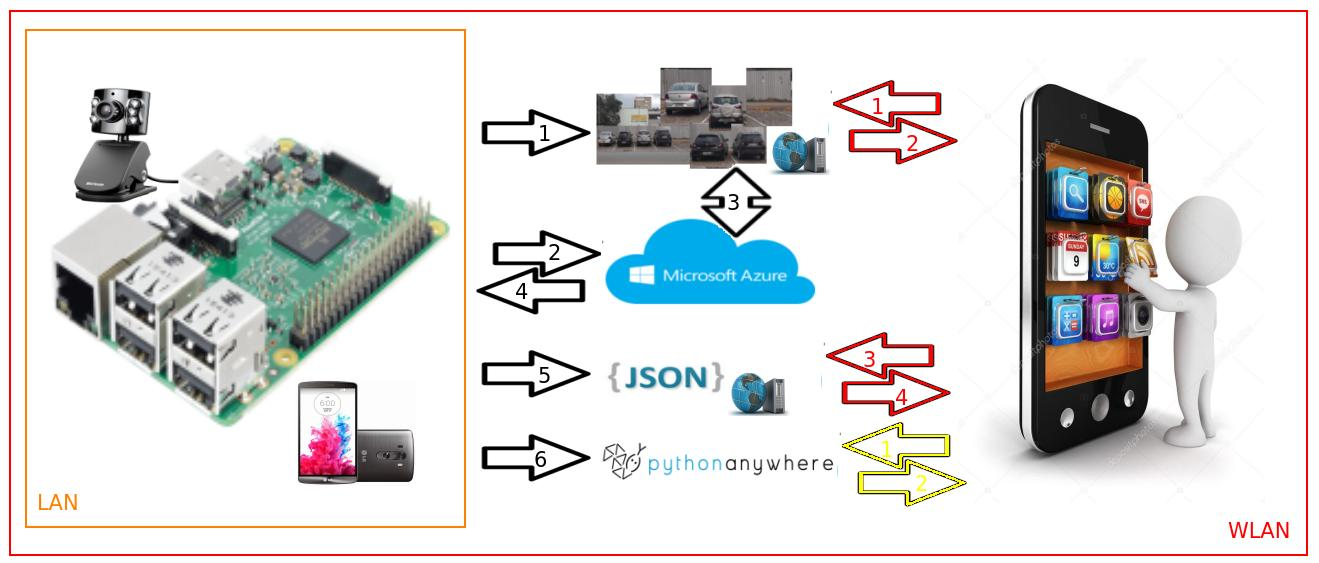
\includegraphics[width=1\textwidth]{img/estrutura.jpeg}   
\end{center}
\begin{itemize}\small
 \item No procedimento, existe uma inconsistência da informação durante uns 30 segundos até 2 min.  
 \item A computer Vision API - Azure é uma boa ferramenta, mas precisa imagens de boa resolução.
 
\end{itemize}

\end{frame}


\begin{frame}{Obrigado!!!}
\begin{center}

\includegraphics[width=.4\textwidth]{img/duvidas.jpg}   
\end{center}
Toda informação e código deste projeto pode ser acessado em:  
\begin{itemize}\small
 \item https://github.com/reynaldocv/IoT-project
\end{itemize}

\end{frame}



\end{document}